%  Copyright (C) 2002 Regents of the University of Michigan, portions used with permission 
%  For more information, see http://csem.engin.umich.edu/tools/swmf
\documentclass[twoside,10pt]{book}
\usepackage{times}
\usepackage{graphicx}
\usepackage{alltt}
\usepackage{amsmath}
\usepackage{epsfig}
\usepackage{fancyhdr}
\usepackage[square]{natbib}
\usepackage{multicol}
\usepackage{subfigure}
\usepackage{fancyvrb}
\usepackage{color}

% use these lengths for a more uniform margin
% this format is more pleasing for stapling
\setlength{\oddsidemargin}{-.1 in}
\setlength{\evensidemargin}{0.0 in}
\setlength{\textwidth}{6.5 in}
\setlength{\topmargin}{0 in}
\setlength{\textheight}{8.5 in}

\renewcommand{\deg}{^{\circ}}


\title{GITM User Manual \\ \large Version 2.1}
\author{A.J. Ridley, A.G. Burrell}

\begin{document}

\pagestyle{fancy}
\lhead[\fancyplain{}{\bfseries\thepage}]{\fancyplain{}{\bfseries\rightmark}}
\rhead[\fancyplain{}{\bfseries\leftmark}]{\fancyplain{}{\bfseries\thepage}}
\cfoot{}

%\pagestyle{headings}

\maketitle

\tableofcontents

\clearpage

%Chapter 1
\chapter{Introduction to GITM}

The Global Ionosphere Thermosphere Model (GITM) is a 3D model of the
upper atmosphere.  It runs for Earth, Mars and Titan.  A version is
being worked on for Jupiter.  GITM solves for the coupled continuity,
momentum and energy equations of the neutrals and ions.  For the ions,
the time rate of change of the velocity is ignored, so the
steady-state ion flow velocity is solved for.  The ion temperature is
a mixture of the electron and neutral temperature.

The neutrals are solved for using the Navier Stokes Equations.  The
continuity equation is solved for for each major species.  One of the
problems with GITM that needs to be rectified is that there are no
real tracer species, so a species is either solved for completely or
is not at all.  These species can still be included in the chemistry
calculation.  There is only one horizontal velocity that is computed,
while there are vertical velocities for each of the major species.  A
bulk vertical velocity is calculated as a mass weighted average.  The
temperature is a bulk temperature.

\section{Source Terms}

Chemistry is the only real source term for the continuity equation.
Typically, diffusion is added in the continuity equation to allow for
eddy diffusion, but this is not the case in GITM.  What happens is
that the vertical velocities are solved for, then a friction term is
applied to that the velocities stay very close together in the eddy
diffusion part of the code.  This way, the velocities can't differ too
much from each other.  Diffusion is not needed, then.

For the horizontal momentum equation, there are the following sources:
(1) ion drag; (2) viscosity; and (3) gravity wave acceleration.  For
the vertical velocity, the source terms are ion drag and friction
between the different neutral species.

For the neutral temperature, the following source terms are included:
(1) radiative cooling; (2) EUV heating; (3) auroral heating; (4) Joule
heating; (5) conduction; and (6) chemical heating.  The biggest pain
for the temperature equation is the use of a normalized temperature.
This means that the {\tt temperature} variable in GITM does not
contain the actual temperature, it contains the temperature multiplies
by Boltzmann's Constant divided by the mean mass.  This turns out to
be a factor that is very similar to the specific heat, or roughly or
order 1000.  In order to get the actual temperature, the variable has
to be multiplied by {\tt temp\_unit}.

\section{Ghost Cells}

GITM is a parallel code.  It uses a 2D domain decomposition, with the
altitude domain being the only thing that is not broken up.  Blocks of
latitude and longitude are used.  These blocks are then distributed
among different processors.  In order to communicate between the
processors, ghostcells are used.  These are cells that essentially
overlap with the neighboring block.  MPI (message passing interface)
is then used to move information from one block to another, filling in
the ghostcells.  The code then loops from 1-N, where the flux is
calculated at the boundaries from the 0-1 boundary to the N-N+1
boundary.  A second order scheme is used to calculate the fluxes,
along with a flux limiter.  Therefore, two ghost cells are needed.

In the vertical direction, ghost cells are also used to set boundary
conditions.  The values in these cells are used to calculate the
fluxes, just as described above.  Different types of boundary
conditions (constant values, constant fluxes, constant gradients,
floating, zero fluxes, etc) can be set by carefully choosing the right
values in the ghost cells.


\label{intro.ch}

\section{Code Outline}
\label{outline.sec}

This is an outline of GITM.  To produce this file, go into the {\tt src} directory, and type:

\begin{verbatim}
cd ../src
./calling_sequence.pl > outline.tex
mv outline.tex ../srcDoc
cd ../srcDoc
\end{verbatim}

{\tt main program} in {\bf main.f90}

\begin{itemize}



\item {\tt init\_mpi}   in file {\bf init\_mpi.f90}
  \begin{itemize}
    \item {\tt MPI\_INIT}
    \item {\tt MPI\_COMM\_RANK}
    \item {\tt MPI\_COMM\_SIZE}
  \end{itemize}


\item {\tt start\_timing}   in file {\bf timing.f90}


\item {\tt delete\_stop}   in file {\bf stop\_file.f90}
  \begin{itemize}
    \item {\tt report} in file library.f90
  \end{itemize}


\item {\tt init\_planet}   in file {\bf ModEarth.f90}
  \begin{itemize}
    \item {\tt time\_int\_to\_real} in file time\_routines.f90
  \end{itemize}


\item {\tt set\_defaults}   in file {\bf ModInputs.f90}
  \begin{itemize}
    \item {\tt set\_strings} in file ModInputs.f90
    \item {\tt time\_int\_to\_real} in file time\_routines.f90
    \item {\tt set\_planet\_defaults} in file Earth.f90
  \end{itemize}


\item {\tt read\_inputs}   in file {\bf read\_inputs.f90}
  \begin{itemize}
    \item {\tt report} in file library.f90
    \item {\tt stop\_gitm} in file library.f90
    \item {\tt stop\_gitm} in file library.f90
    \item {\tt stop\_gitm} in file library.f90
    \item {\tt MPI\_Bcast}
    \item {\tt stop\_gitm} in file library.f90
    \item {\tt MPI\_Bcast}
    \item {\tt stop\_gitm} in file library.f90
  \end{itemize}


\item {\tt set\_inputs}   in file {\bf set\_inputs.f90}
  \begin{itemize}
    \item {\tt report} in file library.f90
    \item {\tt read\_in\_int} in file set\_inputs.f90
    \item {\tt time\_int\_to\_real} in file time\_routines.f90
    \item {\tt time\_real\_to\_int} in file time\_routines.f90
    \item {\tt fix\_vernal\_time} in file set\_inputs.f90
    \item {\tt read\_in\_int} in file set\_inputs.f90
    \item {\tt time\_int\_to\_real} in file time\_routines.f90
    \item {\tt read\_in\_time} in file set\_inputs.f90
    \item {\tt read\_in\_int} in file set\_inputs.f90
    \item {\tt read\_in\_real} in file set\_inputs.f90
    \item {\tt read\_in\_logical} in file set\_inputs.f90
    \item {\tt read\_in\_real} in file set\_inputs.f90
    \item {\tt read\_in\_real} in file set\_inputs.f90
    \item {\tt time\_real\_to\_int} in file time\_routines.f90
    \item {\tt read\_in\_real} in file set\_inputs.f90
    \item {\tt read\_in\_real} in file set\_inputs.f90
    \item {\tt IO\_set\_f107\_single}
    \item {\tt IO\_set\_f107a\_single}
    \item {\tt read\_in\_logical} in file set\_inputs.f90
    \item {\tt read\_in\_logical} in file set\_inputs.f90
    \item {\tt read\_in\_real} in file set\_inputs.f90
    \item {\tt read\_in\_real} in file set\_inputs.f90
    \item {\tt read\_in\_real} in file set\_inputs.f90
    \item {\tt read\_in\_real} in file set\_inputs.f90
    \item {\tt read\_in\_real} in file set\_inputs.f90
    \item {\tt read\_in\_logical} in file set\_inputs.f90
    \item {\tt read\_in\_logical} in file set\_inputs.f90
    \item {\tt read\_in\_logical} in file set\_inputs.f90
    \item {\tt read\_in\_logical} in file set\_inputs.f90
    \item {\tt read\_in\_logical} in file set\_inputs.f90
    \item {\tt read\_in\_logical} in file set\_inputs.f90
    \item {\tt read\_in\_real} in file set\_inputs.f90
    \item {\tt IO\_set\_hpi\_single}
    \item {\tt read\_in\_real} in file set\_inputs.f90
    \item {\tt IO\_set\_kp\_single}
    \item {\tt read\_in\_real} in file set\_inputs.f90
    \item {\tt read\_in\_real} in file set\_inputs.f90
    \item {\tt read\_in\_real} in file set\_inputs.f90
    \item {\tt read\_in\_real} in file set\_inputs.f90
    \item {\tt read\_in\_real} in file set\_inputs.f90
    \item {\tt IO\_set\_imf\_by\_single}
    \item {\tt IO\_set\_imf\_bz\_single}
    \item {\tt IO\_set\_sw\_v\_single}
    \item {\tt read\_in\_string} in file set\_inputs.f90
    \item {\tt IO\_set\_inputs}
    \item {\tt read\_MHDIMF\_Indices}
    \item {\tt read\_in\_logical} in file set\_inputs.f90
    \item {\tt read\_in\_logical} in file set\_inputs.f90
    \item {\tt read\_in\_logical} in file set\_inputs.f90
    \item {\tt read\_in\_logical} in file set\_inputs.f90
    \item {\tt read\_in\_logical} in file set\_inputs.f90
    \item {\tt read\_in\_logical} in file set\_inputs.f90
    \item {\tt read\_in\_string} in file set\_inputs.f90
    \item {\tt read\_in\_string} in file set\_inputs.f90
    \item {\tt read\_in\_string} in file set\_inputs.f90
    \item {\tt read\_in\_real} in file set\_inputs.f90
    \item {\tt read\_in\_int} in file set\_inputs.f90
    \item {\tt read\_in\_int} in file set\_inputs.f90
    \item {\tt read\_in\_real} in file set\_inputs.f90
    \item {\tt read\_in\_logical} in file set\_inputs.f90
    \item {\tt read\_in\_logical} in file set\_inputs.f90
    \item {\tt read\_in\_logical} in file set\_inputs.f90
    \item {\tt read\_in\_logical} in file set\_inputs.f90
    \item {\tt read\_in\_logical} in file set\_inputs.f90
    \item {\tt read\_in\_logical} in file set\_inputs.f90
    \item {\tt read\_in\_logical} in file set\_inputs.f90
    \item {\tt read\_in\_logical} in file set\_inputs.f90
    \item {\tt read\_in\_logical} in file set\_inputs.f90
    \item {\tt read\_in\_real} in file set\_inputs.f90
    \item {\tt read\_in\_real} in file set\_inputs.f90
    \item {\tt read\_in\_logical} in file set\_inputs.f90
    \item {\tt read\_in\_logical} in file set\_inputs.f90
    \item {\tt read\_in\_real} in file set\_inputs.f90
    \item {\tt read\_in\_logical} in file set\_inputs.f90
    \item {\tt read\_in\_logical} in file set\_inputs.f90
    \item {\tt read\_in\_logical} in file set\_inputs.f90
    \item {\tt read\_in\_logical} in file set\_inputs.f90
    \item {\tt read\_in\_real} in file set\_inputs.f90
    \item {\tt read\_in\_real} in file set\_inputs.f90
    \item {\tt read\_in\_real} in file set\_inputs.f90
    \item {\tt read\_in\_logical} in file set\_inputs.f90
    \item {\tt read\_in\_logical} in file set\_inputs.f90
    \item {\tt read\_in\_logical} in file set\_inputs.f90
    \item {\tt read\_in\_logical} in file set\_inputs.f90
    \item {\tt read\_in\_logical} in file set\_inputs.f90
    \item {\tt read\_in\_logical} in file set\_inputs.f90
    \item {\tt read\_in\_logical} in file set\_inputs.f90
    \item {\tt read\_in\_real} in file set\_inputs.f90
    \item {\tt read\_in\_int} in file set\_inputs.f90
    \item {\tt read\_in\_real} in file set\_inputs.f90
    \item {\tt read\_in\_logical} in file set\_inputs.f90
    \item {\tt read\_in\_logical} in file set\_inputs.f90
    \item {\tt read\_in\_logical} in file set\_inputs.f90
    \item {\tt read\_in\_logical} in file set\_inputs.f90
    \item {\tt read\_in\_logical} in file set\_inputs.f90
    \item {\tt read\_in\_logical} in file set\_inputs.f90
    \item {\tt read\_in\_logical} in file set\_inputs.f90
    \item {\tt read\_in\_logical} in file set\_inputs.f90
    \item {\tt read\_in\_string} in file set\_inputs.f90
    \item {\tt read\_in\_string} in file set\_inputs.f90
    \item {\tt read\_in\_real} in file set\_inputs.f90
    \item {\tt read\_in\_real} in file set\_inputs.f90
    \item {\tt read\_in\_real} in file set\_inputs.f90
    \item {\tt read\_in\_real} in file set\_inputs.f90
    \item {\tt read\_in\_real} in file set\_inputs.f90
    \item {\tt read\_in\_logical} in file set\_inputs.f90
    \item {\tt read\_in\_real} in file set\_inputs.f90
    \item {\tt read\_in\_real} in file set\_inputs.f90
    \item {\tt read\_in\_logical} in file set\_inputs.f90
    \item {\tt read\_in\_int} in file set\_inputs.f90
    \item {\tt read\_in\_int} in file set\_inputs.f90
    \item {\tt read\_in\_real} in file set\_inputs.f90
    \item {\tt read\_in\_real} in file set\_inputs.f90
    \item {\tt read\_in\_real} in file set\_inputs.f90
    \item {\tt read\_in\_real} in file set\_inputs.f90
    \item {\tt read\_in\_real} in file set\_inputs.f90
    \item {\tt read\_in\_real} in file set\_inputs.f90
    \item {\tt read\_in\_real} in file set\_inputs.f90
    \item {\tt read\_in\_logical} in file set\_inputs.f90
    \item {\tt read\_in\_logical} in file set\_inputs.f90
    \item {\tt read\_in\_time} in file set\_inputs.f90
    \item {\tt read\_in\_time} in file set\_inputs.f90
    \item {\tt read\_in\_real} in file set\_inputs.f90
    \item {\tt read\_in\_logical} in file set\_inputs.f90
    \item {\tt read\_in\_real} in file set\_inputs.f90
    \item {\tt read\_in\_int} in file set\_inputs.f90
    \item {\tt read\_in\_string} in file set\_inputs.f90
    \item {\tt read\_in\_real} in file set\_inputs.f90
    \item {\tt read\_in\_int} in file set\_inputs.f90
    \item {\tt read\_in\_string} in file set\_inputs.f90
    \item {\tt read\_in\_real} in file set\_inputs.f90
    \item {\tt read\_satellites} in file satellites.f90
    \item {\tt read\_in\_real} in file set\_inputs.f90
    \item {\tt read\_in\_real} in file set\_inputs.f90
    \item {\tt read\_in\_real} in file set\_inputs.f90
    \item {\tt read\_in\_logical} in file set\_inputs.f90
    \item {\tt read\_in\_string} in file set\_inputs.f90
    \item {\tt read\_in\_string} in file set\_inputs.f90
    \item {\tt read\_in\_real} in file set\_inputs.f90
    \item {\tt read\_in\_logical} in file set\_inputs.f90
    \item {\tt read\_in\_string} in file set\_inputs.f90
    \item {\tt Set\_Euv} in file calc\_euv.f90
    \item {\tt read\_in\_logical} in file set\_inputs.f90
    \item {\tt read\_in\_real} in file set\_inputs.f90
    \item {\tt read\_in\_string} in file set\_inputs.f90
    \item {\tt IO\_set\_inputs}
    \item {\tt read\_NGDC\_Indices}
    \item {\tt read\_in\_string} in file set\_inputs.f90
    \item {\tt read\_in\_string} in file set\_inputs.f90
    \item {\tt IO\_set\_inputs}
    \item {\tt read\_SWPC\_Indices}
    \item {\tt read\_in\_string} in file set\_inputs.f90
    \item {\tt IO\_set\_inputs}
    \item {\tt read\_NOAAHPI\_Indices}
    \item {\tt stop\_gitm} in file library.f90
    \item {\tt time\_int\_to\_real} in file time\_routines.f90
  \end{itemize}


\item {\tt initialize\_gitm}   in file {\bf initialize.f90}
  \begin{itemize}
    \item {\tt init\_radcooling} in file ModEarth.f90
    \item {\tt start\_timing} in file timing.f90
    \item {\tt report} in file library.f90
    \item {\tt time\_real\_to\_int} in file time\_routines.f90
    \item {\tt fix\_vernal\_time} in file set\_inputs.f90
    \item {\tt get\_f107}
    \item {\tt get\_f107a}
    \item {\tt init\_grid} in file init\_grid.f90
    \item {\tt read\_inputs} in file read\_inputs.f90
    \item {\tt set\_inputs} in file set\_inputs.f90
    \item {\tt read\_restart} in file restart.f90
    \item {\tt init\_msis} in file init\_msis.Earth.f90
    \item {\tt set\_RrTempInd} in file ModRates.Earth.f90
    \item {\tt init\_euv} in file calc\_euv.f90
    \item {\tt init\_altitude} in file init\_altitude.f90
    \item {\tt UAM\_gradient}
    \item {\tt init\_heating\_efficiency} in file Earth.f90
    \item {\tt init\_magheat} in file ModEarth.f90
    \item {\tt init\_isochem} in file Mars.f90
    \item {\tt init\_aerosol} in file ModEarth.f90
    \item {\tt init\_isochem} in file Mars.f90
    \item {\tt init\_msis} in file init\_msis.Earth.f90
    \item {\tt get\_temperature} in file init\_altitude.f90
    \item {\tt init\_iri} in file init\_iri.Earth.f90
    \item {\tt read\_waccm\_tides} in file tides.f90
    \item {\tt update\_waccm\_tides} in file tides.f90
    \item {\tt read\_tides} in file tides.f90
    \item {\tt update\_tides} in file tides.f90
    \item {\tt init\_b0} in file init\_b0.f90
    \item {\tt init\_energy\_deposition} in file init\_energy\_deposition.f90
    \item {\tt report} in file library.f90
    \item {\tt SUBSOLR}
    \item {\tt exchange\_messages\_sphere} in file exchange\_messages\_sphere.f90
    \item {\tt calc\_pressure} in file calc\_pressure.f90
    \item {\tt UA\_calc\_electrodynamics} in file calc\_electrodynamics.f90
    \item {\tt calc\_eddy\_diffusion\_coefficient} in file Earth.f90
    \item {\tt calc\_rates} in file calc\_rates.Earth.f90
    \item {\tt calc\_viscosity} in file calc\_rates.Earth.f90
    \item {\tt calc\_rates} in file calc\_rates.Earth.f90
    \item {\tt end\_timing} in file timing.f90
    \item {\tt calc\_vtec} in file calc\_tec.f90
    \item {\tt calc\_single\_vtec} in file calc\_tec.f90
  \end{itemize}


\item {\tt write\_output}   in file {\bf write\_output.f90}
  \begin{itemize}
    \item {\tt output} in file output\_common.f90
    \item {\tt move\_satellites} in file satellites.f90
    \item {\tt write\_restart} in file restart.f90
    \item {\tt logfile} in file logfile.f90
  \end{itemize}


\item {\tt report}   in file {\bf library.f90}


\item Loop Start
  \begin{itemize}


  \item {\tt calc\_pressure}   in file {\bf calc\_pressure.f90}
    \begin{itemize}
      \item {\tt report} in file library.f90
    \end{itemize}


  \item {\tt calc\_timestep\_vertical}   in file {\bf calc\_timestep.f90}
    \begin{itemize}
      \item {\tt report} in file library.f90
      \item {\tt MPI\_AllREDUCE}
      \item {\tt stop\_gitm} in file library.f90
    \end{itemize}


  \item {\tt calc\_timestep\_horizontal}   in file {\bf calc\_timestep.f90}
    \begin{itemize}
      \item {\tt report} in file library.f90
      \item {\tt MPI\_AllREDUCE}
    \end{itemize}


  \item {\tt advance}   in file {\bf advance.f90}
    \begin{itemize}
      \item {\tt report} in file library.f90
      \item {\tt start\_timing} in file timing.f90
      \item {\tt update\_tides} in file tides.f90
      \item {\tt update\_waccm\_tides} in file tides.f90
      \item {\tt advance\_vertical\_all} in file advance.f90
      \item {\tt add\_sources} in file add\_sources.f90
      \item {\tt advance\_horizontal\_all} in file advance.f90
      \item {\tt time\_real\_to\_int} in file time\_routines.f90
      \item {\tt get\_f107}
      \item {\tt stop\_gitm} in file library.f90
      \item {\tt get\_f107a}
      \item {\tt stop\_gitm} in file library.f90
      \item {\tt init\_msis} in file init\_msis.Earth.f90
      \item {\tt init\_iri} in file init\_iri.Earth.f90
      \item {\tt init\_b0} in file init\_b0.f90
      \item {\tt end\_timing} in file timing.f90
      \item {\tt report} in file library.f90
      \item {\tt start\_timing} in file timing.f90
      \item {\tt calc\_rates} in file calc\_rates.Earth.f90
      \item {\tt calc\_viscosity} in file calc\_rates.Earth.f90
      \item {\tt advance\_vertical} in file advance\_vertical.f90
      \item {\tt end\_timing} in file timing.f90
      \item {\tt report} in file library.f90
      \item {\tt start\_timing} in file timing.f90
      \item {\tt exchange\_messages\_sphere} in file exchange\_messages\_sphere.f90
      \item {\tt calc\_rates} in file calc\_rates.Earth.f90
      \item {\tt calc\_physics} in file calc\_physics.f90
      \item {\tt advance\_horizontal} in file advance\_horizontal.f90
      \item {\tt calc\_physics} in file calc\_physics.f90
      \item {\tt calc\_rates} in file calc\_rates.Earth.f90
      \item {\tt advance\_horizontal} in file advance\_horizontal.f90
      \item {\tt exchange\_messages\_sphere} in file exchange\_messages\_sphere.f90
      \item {\tt end\_timing} in file timing.f90
    \end{itemize}


  \item {\tt check\_stop}   in file {\bf stop\_file.f90}
    \begin{itemize}
      \item {\tt report} in file library.f90
      \item {\tt start\_timing} in file timing.f90
      \item {\tt MPI\_AllREDUCE}
      \item {\tt check\_start} in file stop\_file.f90
      \item {\tt end\_timing} in file timing.f90
    \end{itemize}


  \item {\tt write\_output}   in file {\bf write\_output.f90}
    \begin{itemize}
      \item {\tt output} in file output\_common.f90
      \item {\tt move\_satellites} in file satellites.f90
      \item {\tt write\_restart} in file restart.f90
      \item {\tt logfile} in file logfile.f90
    \end{itemize}


  \end{itemize} %loop 


 \item Loop End


\item {\tt finalize\_gitm}   in file {\bf finalize.f90}
  \begin{itemize}
    \item {\tt UA\_calc\_electrodynamics} in file calc\_electrodynamics.f90
    \item {\tt output} in file output\_common.f90
    \item {\tt write\_restart} in file restart.f90
    \item {\tt end\_timing} in file timing.f90
    \item {\tt report\_timing} in file timing.f90
    \item {\tt UAM\_XFER\_destroy} in file ModSphereInterface.f90
    \item {\tt UAM\_write\_error} in file ModSphereInterface.f90
    \item {\tt stop\_gitm} in file library.f90
    \item {\tt MPI\_FINALIZE}
  \end{itemize}


\item {\tt stop\_gitm}   in file {\bf library.f90}
  \begin{itemize}
    \item {\tt CON\_stop} in file main.f90
    \item {\tt MPI\_abort}
  \end{itemize}
\end{itemize}


%Chapter 2
\chapter{Getting Started}
\label{quickstart.ch}
\section{Extracting the code from a tar file}

Create a new and empty directory, and open the tar file you received,
e.g.:
\begin{verbatim}
mkdir Gitm 
cd Gitm 
mv ../gitm.tgz . 
tar -xvzf gitm.tgz 
\end{verbatim}

\section{Checking out the code with CVS}

If CVS (Concurrent Versions System) is available on your computer and
you have an account on the CVS server machine herot.engin.umich.edu,
you can use CVS to install the current or a particular version of the
code. First of all have the following environment variables:
\begin{verbatim}
setenv CVSROOT UserName@herot.engin.umich.edu:/CVS/FRAMEWORK
setenv CVS_RSH ssh
\end{verbatim}
where UserName is your user name on herot. Here it is assumed that you
use csh or tcsh. Also put these settings into your .cshrc file so it
is automatically executed at login. Alternatively, use
\begin{verbatim}
CVSROOT=UserName@herot.engin.umich.edu:/CVS/FRAMEWORK 
export CVSROOT 
CVS_RSH=ssh 
export CVS_RSH
\end{verbatim}
under sh, ksh and bash shells, and also put these commands into your
.bashrc or .profile file so it is automatically executed at login.

Once the CVS environment variables are set, you can download the
current (HEAD) version of the GITM distribution with
\begin{verbatim}
cvs checkout GITM2
\end{verbatim}

If you want a particular version, use
\begin{verbatim}
cvs checkout -r v2_0 GITM2
\end{verbatim}
where v2\_0 is the it tag associated with the version. To download bug
fixes or new features, the
\begin{verbatim}
cvs update 
\end{verbatim}
command can be used. See {\tt man cvs} for more information.

A lot of times, you don't really want the {\tt GITM2} directory to
stay that name, since you might download a couple different version
(maybe one for development and one for runs).  Therefore, typically
you will:
\begin{verbatim}
mv GITM2 GITM2.Development
\end{verbatim}

\section{Configuring and Making GITM}

In order to compile GITM, you have to configure it first.  The
configure script is inherited from the Space Weather Modeling
Framework.  There are two primary reasons you need to do the
configure: (1) put the right {\tt Makefile} in the right place,
specifying the compiler and the version of MPI that you will use to
link the code; (2) put the right MPI header in the right place.  It
also does some things like hard-codes the path of the source code into
the {\tt Makefile}. Currently the configure script is not capable of detecting the system and compilers available.  Some examples for commonly used set-ups are shown below.

Installing on Nyx:
\begin{verbatim}
./Config.pl -install -compiler=ifortmpif90 -earth
\end{verbatim}

Installing on a Mac with gfortran and openmpi:
\begin{verbatim}
./Config.pl -install -compiler=gfortran -earth
\end{verbatim}

Installing on a computer with gfortran and not using MPI:
\begin{verbatim}
./Config.pl -install -compiler=gfortran -earth -nompi
\end{verbatim}

Sometimes people have a hard time with the ModUtilities.F90 file.  If
you have errors with this file, try (for example):
\begin{verbatim}
./Config.pl -uninstall
./Config.pl -install -compiler=gfortran -earth -noflush
\end{verbatim}

Don't forget, after configuring the Makefiles, you must still compile the code!
\begin{verbatim}
make
make test_earth
make install
\end{verbatim}

\section{Running the Code}

GITM requires a bunch of files to be in the right place in order to
run.  Therefore, it is best to use the makefile to create a run
directory:
\begin{verbatim}
make rundir
mv run myrun
\end{verbatim}
where {\tt myrun} can be whatever you want.  I will use {\tt
myrun} as an example.  You can actually put this directory where ever
you want.  On many systems (such as nyx), there is a {\tt nobackup} scratch disk that
you are supposed to use for runs, instead of your home directory.  If you need to ensure that your home directory doesn't use too much space, moving the run directory onto a disk with more free space can solve the problem:

\begin{verbatim}
make rundir
mv run /nobackup/myaccount/gitm/myrun
ln -s /nobackup/myaccount/gitm/myrun .
\end{verbatim}

This creates a shortcut to the {\tt myrun} directory location on {\tt nobackup} in your GITM working directory.  It allows you to treat the run directory as if it were a local directory, but it isn't!  It also means that you don't have to compile and install GITM on the scratch disk, where program storage may not be allowed.

Once you have created the run directory, you can run the default simulation, by:

\begin{verbatim}
cd myrun
mpirun -np 4 GITM.exe
\end{verbatim}
This, hopefully should run GITM for Earth for 5 minutes.  If it
doesn't work, then you might have mpi set up incorrectly.  The default
is to allow you to run 4 blocks per processor, and the default {\tt
UAM.in} file is set up for 4 blocks, so you could try just running
GITM without mpi, just to see if it works at all:
\begin{verbatim}
./GITM.exe
\end{verbatim}
If that doesn't work, then it probably didn't compile correctly.
Hopefully, it just worked!

\section{Post Processing}
\label{post_process.sec}

GITM, by default, produces one file per block per output.  If you are outputting often and you are running with many blocks, you can produce a huge number of files.  To post process all of these files, simply:

\begin{verbatim}
cd UA
./pGITM
\end{verbatim}

This merges all of the files for one time period, for one file type into the same file.  You can actually running this while the code is running, since GITM doesn't use old files, unless you are using the APPENDFILE option.  As implied by the option's name, APPENDFILE opens an existing file and appends the most recent data to it.  This feature is typically used only when running a satellite track though GITM.  More information on the APPENDFILE option is located in Chapter~\ref{input.ch} Section~\ref{def_out.sec}.

If you are NOT using satellites and NOT using APPENDFILE, then you are free and clear to use pGITM as often as you want during a run.  To avoid deleting a file that GITM is currently writing to, it is recommended that pGITM be run as part of a script in which there is a five minute pause between executions.

Another useful script, when running GITM on another system, is given in the block below.  It occasionally executes an rsync between the computer that you run GITM on and your home computer.  This allows you to bring over and evaluate the output files as they become available.  To do this, execute pGITM at a set cadence (60 seconds in the example) while GITM is running and then rsync the remote and home directories (excluding all unprocessed files).  Finally, remove the processed and rsynced files to prevent the remote directory from filling up.  Be sure to replace yourname@home.computer with your user and computer names!  This is a very simple, but very useful script.

\begin{verbatim}
#!/bin/csh
rm -f stop
set LOC=$1

if (-f remoteloc) set LOC=`cat remoteloc`

while (!(-f stop))
  rsync -vrae ssh log.* UAM.* imf* yourname@home.computer:$LOC
  cd UA ; ./pGITM ; rsync --exclude '*.[bsh][0123ae][0123456789at]*' -vrae ssh d
ata yourname@home.computer:$LOC ; cd ..
  sleep 60
end
\end{verbatim}

\section{The Code Won't Compile!!}
I'm sorry. I tried to make this work on many different platforms, but
sometimes machines are very specific, and it just doesn't work out of
the box. Here are some ideas on how to quickly get this thing
compiling.

\subsubsection{Can't find the right Makefile.whatever}

If make does not work, then there is probably a problem with not
finding the FORTRAN 90 compiler. The platform and machine specific
Makefiles are in srcMake. If you type:
\begin{verbatim}
uname 
ls srcMake
\end{verbatim}

If you don't see a file named something like Makefile.uname (where
uname is the output of the uname command), then you will have to build
a proper general Makefile.

You will need a little a little information about your computer, like
what the mpif90 compiler is called and where it is located. Take a
look at srcMake/Makefile.Linux, and try to figure out what all of the
flags are for your system. Then create a srcMake/Makefile.uname with
the correct information in it.

\subsubsection{The compiler doesn't recognize flag -x}

You have an operating system that is recognized, but probably a
different compiler. In the srcMake/Makefile.uname file (where uname is
the output of the uname command), there is a line:

OSFLAGS	= -w -dusty

You need to change this line to something more appropriate for your
compiler. Try deleting the flags and compile. If that doesn't work,
you will have to check the man pages of your compiler.

\subsubsection{src/ModHwm.90 doesn't compile}

Certain versions of gfortran (4.6 and later) may give the following error:

\begin{verbatim}
src/ModHwm.f90:168.22:

        call HWMupdate(input,last,gfs,gfl,gfm,gvbar,gwbar,gbz,gbm,gzwght,glev,u
                      1
Error: Dummy argument 'ebz' of procedure 'hwmupdate' at (1) has an attribute
 that requires an explicit interface for this procedure

src/ModHwm.f90:168.22:

        call HWMupdate(input,last,gfs,gfl,gfm,gvbar,gwbar,gbz,gbm,gzwght,glev,u
                      1
Error: Dummy argument 'ebz' of procedure 'hwmupdate' at (1) has an attribute
 that requires an explicit interface for this procedure
\end{verbatim}

This is caused by the inputs in HWM.  The latest incarnations of gfortran don't allow optional inputs that are not declared.  More information about this can be found at:

\begin{verbatim}
http://cosmocoffee.info/viewtopic.php?p=5136
\end{verbatim}

A solution to this problem is currently being sought.


%Chapter 3
\chapter{Inputs}
\label{input.ch}
\section{Principle Input}
\label{uam.sec}

{\tt UAM.in} contains the majority of the variables that can be changed in a GITM run.  Very few of these input options are required as input, all other options will default to values specified by the ModInputs.f90 subroutine, which can be found in the {\tt src} directory.  Example {\tt UAM.in} files for various types of runs are made available in the {\tt srcData} directory.

This input file can be altered at will without the need to recompile the code either ``by hand" or using a script such as {\tt makerun.pl}.  This script, which is located on {\tt harot.engin.umich.edu:/bigdisk1/bin}, takes command line input to create a UAM.in file and any desired auxiliary files, discussed in more detail in section~\ref{aux.sec}, using locally stored data.

The following sections present the GITM input options grouped by type.  This is not the order you will find them in a typical {\tt UAM.in} file or the order you will find the input processed in {\tt ModInputs.f90}.  This reinforces the flexibility of the input file, which doesn't care what order the input options are specified with one exception.  The starting and ending times (discussed in section~\ref{required.sec}) \textit{must} be defined before any solar or geomagnetic indices (discussed in section~\ref{indices.sec}).  It is probably a good practice to begin any {\tt UAM.in} file either with the output options (discussed in section~\ref{def_out.sec}) or the starting and ending times.

%%

\subsection{Required Inputs}
\label{required.sec}

The only inputs that must be specified are the starting and ending times.  These times are specified using universal time blocks that specify the date (A.D.) and time of day.  Remember, these two blocks must be specified before any of the solar or geomagnetic index blocks, outlined in section~\ref{indices.sec}.

\subsubsection{TIMESTART}
\label{starttime.sec}

This input block sets the starting time of the simulation.  Although the input time can be defined down to the second, construction scripts will ignore temporal units smaller than a day since a lead time of a day is typically desired for any model run.  Shorter runs should only used to test the model compilation.

GITM can be set to restart after pausing.  This has no effect on TIMESTART, these values should always contain the real starting time, not the restart time.

\begin{verbatim}
#TIMESTART
(integer) year   
(integer) month 
(integer) day    
(integer) hour    
(integer) minute 
(integer) second
\end{verbatim}

\subsubsection{TIMEEND}
\label{endtime.sec}

This input block sets the ending time of the simulation.  As mentioned above, GITM runs typically last a minimum of two days (with one day as start-up to allow the processes to settle into equilibrium) and so the hour, minute, and second options are commonly ignored.

\begin{verbatim}
#TIMEEND
(integer) year    
(integer) month
(integer) day     
(integer) hour    
(integer) minute  
(integer) second  
\end{verbatim}

%%

\subsection{Temporal Boundaries}
\label{time.sec}

The input options described here are optional and used to set the temporal boundaries in GITM, including the processing times.

\subsubsection{PAUSETIME}
\label{pausetime.sec}

This input option sets a time for the code to pause.  There is no good reason to use this option.

\begin{verbatim}
#PAUSETIME
(integer) year
(integer) month 
(integer) day 
(integer) hour 
(integer) minute 
(integer) second
\end{verbatim}

\subsubsection{CPUTIMEMAX}
\label{cputimemax.sec}

This sets the maximum CPU time that the code should run before it starts to write a restart file and end the simulation.  It is very useful on systems that have a queueing system and has limited time runs.  Typically, set it for a couple of minutes short of the maximum wall clock, since it needs some time to write the restart files.

\begin{verbatim}
#CPUTIMEMAX
(real) CPUTimeMax
\end{verbatim}

\subsubsection{CFL}
\label{cfl.sec}

The CFL option defines how large a time step GITM will take.  This is set as a fraction of the maximum time step, so 1.0 is the maximum value, while 0.75 is a typical value.  If instabilities form during a model run, lowering this option is a good first step to take.

\begin{verbatim}
#CFL
(real) cfl
\end{verbatim}

\subsection{Defining Outputs}
\label{def_out.sec}

The input option blocks described here are used to specify the level and type of verboseness. 

\subsubsection{LOGFILE}
\label{logfile.sec}

Log files are very important and the LOGFILE input option allows the user to control how much information the GITM logfile will contain.  This logfile is output into the {\tt UA/data/} directory in a file following a naming convention like {\tt log*.dat}.  Although you can output the log file at whatever frequency you would like, setting the time-step to some very small value will allow GITM to produce a log output every iteration, which is a good thing.  DtLogFile specifies this time-step in seconds.

\begin{verbatim}
#LOGFILE
(real) DtLogFile
\end{verbatim}

\subsubsection{DEBUG}
\label{debug.sec}

This will set the level of GITM's verboseness.  Set the iDebugLevel to 0 for minimal output and to 10 to retrieve \textit{everything}.  You can also limit output to a specific processor using iDebugProc.  The processors are named PE x, where PE indicates that you are tagging a processor and x is the zero offset integer indicating the processor number.  So ``PE 0" would indicate that output from the first processor is desired.

If you set the iDebugLevel to 0 (the default), you can set the debug report time step using DtReport.  This time step is given in seconds.  The final keyword in this input option, UseBarriers, forces the different nodes running the GITM code to sync up with each other frequently when employed.

\begin{verbatim}
#DEBUG
(integer) iDebugLevel
(integer) iDebugProc  
(real) DtReport    
(logical) UseBarriers 
\end{verbatim}

\subsubsection{SATELLITES}
\label{satellites.sec}

To improve model-data studies, GITM can output model results along the satellite paths.  Any number of satellites may be flown through a GITM simulation.  Output from the satellite paths is provided at the specified universal time, geographic latitude and longitude.  Instead of confining the model output to the satellite altitude, simulated output is provided over the entire GITM altitude range.

\begin{verbatim}
#SATELLITES
(integer) nSats
(string) SatFile(n)
(real) DtPlot(n)
\end{verbatim}
\vspace{-.1in}
\hspace{.6in} $\vdots$
\vspace{.1in}

To fly several satellites through GITM, the user must set nSats, SatFile(n), and DtPlot(n) for each satellite.  nSats specifies the number of satellites, SatFile(n) gives the name of the satellite flight path file (discussed in more detail in section~\ref{sat_aux.sec}), and DtPlot(n) specifies the time-step for the GITM satellite output in seconds.  The following verbatim block shows the arrangement for two satellites.

\begin{verbatim}
#SATELLITES
2 nSats
grace.sat SatFile1
1 DtPlot1
champ.sat SatFile2
1 DtPlot2
\end{verbatim}

\subsubsection{APPENDFILES}
\label{appendfiles.sec}

GITM defaults to creating many output files for satellite runs, but this option tells GITM to create just one single file per satellite.  This makes GITM output significantly less files.  In the future, this option may be available for other types of output as well.

\begin{verbatim}
#APPENDFILES
(logical) DoAppendFiles
\end{verbatim}

\subsubsection{SAVEPLOT}
\label{saveplot.sec}

This input option specifies the types of files GITM will output.  The most common type is 3DALL, which outputs all primary state variables. Types (specified in OutputType) include : 3DALL, 3DNEU, 3DION, 3DTHM, 3DCHM, 3DUSR, 3DGLO, 2DGEL, 2DMEL, 2DUSR, 2DTEC, 1DALL, 1DGLO, 1DTHM, 1DNEW, 1DCHM, 1DCMS, and 1DUSR.  These file types specify the number of dimensions (3D, 2D, 1D) in which GITM may be run and the different primary state variables that are included in the output (NEU stands for neutrals, ION stands for ionosphere, THM stands for thermosphere, CHM stands for BLAH, USR stands for BLAH, GLO stands for day glow, TEC stands for total electron content, GEL stands for global electric BLAH, and MEL stands for BLAH).  Any number of output files may be produced, but nOutputTypes must be used to specify the number of types to be created and an OutputType and DtPlot must be provided for each output just as was done for multiple satellites.  DtRestart and DtPlot specify the time-step in seconds for producing restart and output files, respectively.  

\begin{verbatim}
#SAVEPLOT
(real) DtRestart
(integer) nOutputTypes 
(string) OutputType
(real) DtPlot   
\end{verbatim}
\vspace{-.1in}
\hspace{.6in} $\vdots$
\vspace{.1in}

\subsubsection{PLOTTIMECHANGE}
\label{plottimechange.sec}

This option allows you to change the output cadence of the files for a limited time.  If you have a short event, such as a solar flare or an eclipse, this options lets you output much more often during the event than during the quiet periods preceding and succeeding the event.

\begin{verbatim}
#PLOTTIMECHANGE
(yyyy mm dd hh mm ss ms) PlotTimeChangeStart
(yyyy mm dd hh mm ss ms) PlotTimeChangeEnd
\end{verbatim}

%%


\subsection{Restart Input}

This section deals with options typically only specified in a restart header.  These options can be used in the principle input file but have very little use if a run does not need to be restarted from a specified point in a previous run.

\subsubsection{RESTART}

Setting this input option to T (true) allows the model to restart from a previous run.

\begin{verbatim}
#RESTART
(logical) DoRestart
\end{verbatim}

\subsubsection{ISTEP}
\label{istep.sec}

This input should not be specified by the user, but is used by the computer to restart after a run has been interrupted.  It gives the iteration number that the model run stopped at.

\begin{verbatim}
#ISTEP
(integer) iStep
\end{verbatim}

\subsubsection{TSIMULATION}

This options sets the offset from the starting time (specified using TIMESTART) to the current simulation time in seconds.  Like ISTEP, this option should really only be used by the computer to restart after a run has been interrupted.

\begin{verbatim}
#TSIMULATION
(real) tsimulation    
\end{verbatim}

%%

\subsection{Numerical Options}
\label{numerical.sec}

The optional inputs in this section allow the user to modify how GITM handles computational scenarios.

\subsubsection{LIMITER}
\label{limiter.sec}

The flux limiter specifies the balance between the model's ability to run robustly and provide realistic gradients.  A realistic atmosphere will occasionally experience sharp changes in characteristics such as electron density.  When GITM attempts to model these variations, the high resolution of the temporal and spatial grids allows the numerical schemes that solve the equations of state to oscillate about the actual value.  One solution to the problem is to err on the side of robustness and require more gradual changes.  This can be done by setting TypeLimiter to minmod or setting TypeLimiter to beta and BetaLimiter to 1.0 (both of these options are the same and the default).  The other solution is to allow sharp changes to occur, realizing that the model will likely overshoot and undershoot and that if an atmospheric characteristic shoots to an unrealistic value the model may crash.

Although there are many different limiter types (see the wikipedia article for a decent introduction: {\tt \\http://en.wikipedia.org/wiki/Flux\_limiter}) GITM uses the Osher function~\citep{Chakravarthy:1983os}, given below in equation~\ref{os.eq}.

\begin{equation}
\label{os.eq}
\phi_{os}(r) = max[0,min(r,\beta)], \;\;\;\; (1 \le \beta \le 2); \;\;\;\; \lim_{r\to\infty} \phi_{os}(r) = \beta
\end{equation}

In this function, $\beta$ is specified by BetaLimiter, and so defaults to the minmod flux limiter function when $\beta = 1$~\citep{roe:1986aa} and to the monotonized central (MC) flux limiter function when $\beta = 2$~\citep{valLeer:1977aa}.

\begin{verbatim}
#LIMITER
(string) TypeLimiter
(real) BetaLimiter
\end{verbatim}

\subsection{Solar and Geomagnetic Indices}
\label{indices.sec}

This section contains the input options that specifies the level of solar and geomagnetic activity.  Recall that these input options must be specified after the starting and ending times (refer to section~\ref{required.sec}) are defined.  Also, note that several of these indices may be specified in different ways.  If you use more than one method to define an index, the last definition will be used.  It is better to just use one method in your {\tt UAM.in} file to avoid confusion.

\subsubsection{F107}
\label{f107.sec}

Sets the F$_{10.7}$ and 81 day average of F$_{10.7}$ (commonly denoted as F$_{10.7a}$ or $\overline{F_{10.7}}$).  This is used to set the range of the initial altitude grid and drive the lower boundary conditions.  It is also used as input into several of the models called by GITM.  The F$_{10.7}$ is a measure of the solar 10.7 cm flux~\citep{Covington:1948aa} and is measured in solar flux units (1 sfu = 10$^{-22}$ W m$^{-2}$ Hz$^{-1}$ = 10,000 jansky).  The F$_{10.7}$ is commonly used as a proxy for the solar EUV output.  

\begin{verbatim}
#F107
(real) f107
(real) f107a
\end{verbatim}

\subsubsection{NGDC\_INDICES}
\label{ngdc_indices.sec}

This input option allows GITM to use an appropriate F$_{10.7}$ for each day that the assimilation runs, instead of a fixed value.  This is accomplished by providing an input file that contains the F$_{10.7}$ values for the entire GITM simulation period and the preceding 81 days.  This allows GITM to compute the appropriate daily F$_{10.7a}$ as well.  Typically, users simply make a file including all F$_{10.7}$ values from 1980 onward, so they never have to worry about missing any preceding days.

\begin{verbatim}
#NGDC_INDICES
(string) filename
\end{verbatim}

\subsubsection{KP}
\label{kp.sec}

The Kp index is not used by GITM, but several models that GITM calls utilize it.  The Kp index is a measure of mid-latitude geomagnetic disturbance and can be obtained from:

 {\tt ftp://ftp.ngdc.noaa.gov/STP/GEOMAGNETIC\_DATA/INDICES/KP\_AP/} 
 
 \noindent while a description of the index can be found at:
 
 {\tt http://www-app3.gfz-potsdam.de/kp\_index/description.html}

\begin{verbatim}
#KP
(real) kp  
\end{verbatim}

\subsubsection{HEMISPHERICPOWER}
\label{hemisphericpower.sec}

This option sets the hemispheric power of the aurora.  Typical values range from 1$-$1000, with 20 being a nominal, quiet time value.

\begin{verbatim}
#HPI
(real) HemisphericPower
\end{verbatim}

\subsubsection{SOLARWIND}
\label{solarwind.sec}

This option is one way to set the driving conditions for the high-latitude electric field models.  Because this option is static and will not change during the run, it is usually better to use the MHD\_INDICES option instead, as MHD\_INDICES provides a dynamic driving environment.

\begin{verbatim}
#SOLARWIND
(real) bx  
(real) by  
(real) bz  
(real) vx  
\end{verbatim}

\subsubsection{MHD\_INDICES}
\label{mhdindices.sec}

Use this option to provide GITM with dynamic IMF and solar wind conditions.  This option can either be omitted entirely; if it is desired a filename whose contents will be discussed in more detail in section~\ref{imf.sec} must be specified.  This file should be located in the same directory as the {\tt UAM.in} file.

\begin{verbatim}
#MHD_INDICES
(string) filename
\end{verbatim}

\subsubsection{EUV\_DATA}
\label{euv.sec}

This input option allows the user to specify the extreme ultraviolet (EUV) flux using solar spectra from any model or data source.  A FISM file~\citep{fism:2007d, fism:2008f} is used as an example in section~\ref{solar_irradiance.sec}.

\begin{verbatim}
#EUV_DATA
(logical) UseEUVData   
(string) cEUVFile     
\end{verbatim}

%%

\subsection{Physical Processes}
\label{physics.sec}

The following options let the user specify how GITM treats different physical boundaries and processes.

\subsubsection{INITIAL}
\label{initial.sec}

This option specifies the initial conditions and the lower boundary conditions.  For Earth, we typically just use MSIS and IRI for initial conditions.  For other planets, the vertical temperature parameters can be set here.  TempMin and TempMax specify the initial temperatures at the bottom and top of the thermosphere in Kelvin, respectively.  TempHeight specifies the height (in kilometers from the surface of the planet) of the midpoint of the temperature gradient.  TempWidth specifies the vertical width (in kilometers) of the temperature gradient. 

\begin{verbatim}
#INITIAL
(logical) UseMSIS
(logical) UseIRI 
If UseMSIS is false (F) then:
(real) TempMin      
(real) TempMax        
(real) TempHeight     
(real) TempWidth     
\end{verbatim}

\subsubsection{STATISTICALMODELSONLY}
\label{statisticalmodelsonly.sec}

There can be benefits to running a simpler ionosphere and thermosphere models.  GITM can be used as a shell to run MSIS and IRI without any coupling.  This input option bypasses GITM and only outputs results from MSIS and IRI.  This option allows the user who is familiar with GITM to get MSIS and IRI output without having to install or know how to run these models independently.  The UseStatisticalModelsOnly flag can be set to {\tt T} or {\tt F} (true or false) and the DtStatisticalModels options lets you specify the time-step (in seconds) used in MSIS and IRI.

\begin{verbatim}
#STATISTICALMODELSONLY
(logical) UseStatisticalModelsOnly
(real) DtStatisticalModels
\end{verbatim}

\subsubsection{TIDES}
\label{tides}

This option uses a series of logical flags to tell GITM how to use tides.   The first flag (UseMSISFlat) tells GITM to use MSIS without tides.  The second flag (UseMSISTides) is using MSIS with full up tides. One of these two flags should be true.  The remaining flags should only be true if UseMSISTides is false, and then only one should be true.  The third flag (UseGSWMTides) uses GSWM tides, while the forth flag (UseWACCMTides) sets GITM to use the WACCM tides.  Essentially, only one tidal model should be used per GITM run.  Information about GSWM can be found at: \\{\tt http://www.hao.ucar.edu/modeling/gswm/gswm.html} and information about WACCM can be found at: \\{\tt http://www.cesm.ucar.edu/working\_groups/WACCM/}.

When running with the MSIS or WACCM tides, no additional input files are needed.  However, when using GSWM additional files must be made accessible to GITM in the {\tt run/UA/DataIn} directory.  These files are stored in the {\tt Tides} directory within GITM.  You can check these files out using CVS (as described in Chapter~\ref{cvs.sec}) and then create links or copy them into your run directory by using: {\tt ln -s ~/GITM/Tides/*bin ~/GITM/run/UA/DataIn/.}

\begin{verbatim}
#TIDES
(logical) UseMSISFlat      
(logical) UseMSISTides      
(logical) UseGSWMTides     
(logical) UseWACCMTides    
\end{verbatim}

\subsubsection{GSWMCOMP}
\label{gswmcomp.sec}

If you decided to use GSWM tides by selecting UseGSWMTides in the TIDES option, you can specify which diurnal and semidiurnal tidal components to include.

\begin{verbatim}
#GSWMCOMP
(logical) GSWMdiurnal(1)        
(logical) GSWMdiurnal(2)       
(logical) GSWMsemidiurnal(1)    
(logical) GSWMsemidiurnal(2)    
\end{verbatim}

\subsubsection{DAMPING}
\label{damping.sec}

This option specifies whether or not to allow damping of the vertical wind oscillations that can occur in the lower atmosphere.

\begin{verbatim}
#DAMPING
(logical) UseDamping        
\end{verbatim}

\subsubsection{GRAVITYWAVE}
\label{gravitywave.sec}
A switch to add heating to the atmosphere.  This was primarily used to explore gravity waves on Titan and has little to no effect on the terrestrial atmosphere.  This options defaults to false.

\begin{verbatim}
#GRAVITYWAVE
(logical) UseGravityWave
\end{verbatim}

\subsubsection{NEWELLAURORA}
\label{newellaurora.sec}

This input option provides several logical flags that allow GITM to use Pat Newell's aurora model, Ovation~\citep{Newell:2002ov}.

\begin{verbatim}
#NEWELLAURORA
(logical) UseNewellAurora   
(logical) UseNewellAveraged 
(logical) UseNewellMono 
(logical) UseNewellWave
(logical) UseNewellRemoveSpikes 
(logical) UseNewellAverage  
\end{verbatim}

\subsubsection{AMIEFILES}
\label{amiefiles.sec}

This option allows the user to specify the electrodynamic state of the polar regions using the Assimilative Mapping of Ionospheric Electrodynamics (AMIE) model~\citep{ridley:2004aa}.  Input files separately specify the conditions at the northern and southern polar caps, and should be in the MIE binary format.  Contact Aaron Ridley for more information about using AMIE with GITM.

\begin{verbatim}
#AMIEFILES
(string) cAMIEFileNorth 
(string) cAMIEFileSouth
\end{verbatim}

\subsubsection{THERMO}
\label{thermo.sec}

This input option sets flags that allow the user to turn various thermospheric processes on and off.  For a realistic run, all three heating flags (for solar, Joule, and auroral heating) should be set to true, along with both cooling flags (for nitrous-oxide, NO, and oxygen, O).  UseConduction, UseUpdatedTurbulentCond, and UseTurbulentCond flag should also all be set to true.  UseDiffusion, however, defaults to false and should not be used for a realistic run.

The only keyword that is not a flag is EddyScaling.  This allows the user to control the Eddy diffusion by applying a multiplicative to the model's Eddy diffusion value.

\begin{verbatim}
#THERMO
(logical) UseSolarHeating   
(logical) UseJouleHeating   
(logical) UseAuroralHeating
(logical) UseNOCooling    
(logical) UseOCooling       
(logical) UseConduction     
(logical) UseTurbulentCond  
(logical) UseUpdatedTurbulentCond
(logical) UseDiffusions
(real) EddyScaling  
\end{verbatim}

\subsubsection{THERMALDIFFUSION}
\label{thermaldiffusion.sec}

This keyword sets the thermal conductivity.  KappaTemp0 should be set to the desired value of the thermal conductivity in MKS units.

\begin{verbatim}
#THERMALDIFFUSION
(real) KappaTemp0
\end{verbatim}

\subsubsection{VERTICALSOURCES}
\label{verticalsources.sec}

This input option provides flags and limits for the vertical thermospheric sources.  The UseEddyInSolver turns the Eddy diffusion on and off, the UseNeutralFrictionInSolver turns the vertical neutral friction on and off, and the MaximumVerticalVelocity sets the limit for vertical neutral winds in meters per second.

\begin{verbatim}
#VERTICALSOURCES
(logical) UseEddyInSolver             
(logical) UseNeutralFrictionInSolver  
(real) MaximumVerticalVelocity    
\end{verbatim}

\subsubsection{EDDYVELOCITY}
\label{eddyvelocity.sec}

This input option further allows the user to specify how Eddy diffusion is treated by providing an flag to use the method presented by~\citet{Boqueho:2005aa}, which was developed for the Martian atmosphere.  The UseEddyCorrection flag is another option that is useful for certain extraterrestrial atmospheres.

\begin{verbatim}
#EDDYVELOCITY
(logical) UseBoquehoAndBlelly 
(logical) UseEddyCorrection
\end{verbatim}

\subsubsection{DIFFUSION}
\label{diffusion.sec}

If you use Eddy diffusion, as indicated by the UseDiffusion flag, you must specify two pressure
levels in units of UNITS using EddyDiffusionPressure[0,1].  Below the first pressure level, the Eddy diffusion will be constant.  Between the first and the second pressure levels, the Eddy diffusion coefficient will drop-off linearly.  Thus, the first pressure must be larger than the second!  The Eddy diffusion coefficient may also be specified using EddyDiffusionCoef.

\begin{verbatim}
#DIFFUSION
(logical) UseDiffusion
(real) EddyDiffusionCoef
(real) EddyDiffusionPressure0 
(real) EddyDiffusionPressure1
\end{verbatim}

\subsubsection{WAVEDRAG}
\label{wavedrag.sec}

This input option allows stress heating to be applied in GITM, providing an additional source of drag in the thermosphere.

\begin{verbatim}
#WAVEDRAG
(logical) UseStressHeating
\end{verbatim}

\subsubsection{FORCING}
\label{forcing.sec}

This input option provides flags for physical processes that drive the thermosphere.

\begin{verbatim}
#FORCING
(logical) UsePressureGradient 
(logical) UseIonDrag          
(logical) UseNeutralFriction  
(logical) UseViscosity        
(logical) UseCoriolis         
(logical) UseGravity        
\end{verbatim}

\subsubsection{IONFORCING}
\label{ionforcing.sec}

This input option turns several ionospheric transport processes on and off.  UseExB turns the {\bf E}$\times${\bf B} plasma drift on and off, UseIonGravity allows the user to determine whether or not to allow the ions to respond to gravity, UseNeutralDrag relegates the forcing from ion-neutral collisions on the ionosphere, and UseIonPressureGradient deals with the ion motions resulting from changes to the plasma pressure gradient.  All of these processes should be on for a realistic simulation.

\begin{verbatim}
#IONFORCING
(logical) UseExB           
(logical) UseIonPressureGradient
(logical) UseIonGravity     
(logical) UseNeutralDrag   
\end{verbatim}

\subsubsection{DYNAMO}
\label{dynamo.sec}

This input option provides flags for the ionospheric dynamo.  The UseDynamo flag turns on a model to calculate the ionospheric electric fields.  DynamoHighLatBoundary sets the polar latitude limit (65$^\circ$ or 70$^\circ$ is a realistic limit), nItersMax sets the maximum number of iterations for the Dynamo convergence (typically set at 500), and the MaxResidual sets the maximum difference, in Volts, to allow between iterations before the value is said to have converged (typically set to 1 V).  The Dynamo currently uses a static high-latitude boundary, though a dynamical one would be ideal.  To get around this, input from AMIE, run using the SuperMag data network, can be used instead of the UseDynamo process.  The use of AMIE input is discussed in section~\ref{amiefiles.sec}.

\begin{verbatim}
#DYNAMO
(logical) UseDynamo   
(real) DynamoHighLatBoundary 
(integer) nItersMax        
(real) MaxResidual     
\end{verbatim}

\subsubsection{ELECTRODYNAMICS}
\label{electrodynamics.sec}

Sets the time-step (in seconds) for updating the high-latitude (and low-latitude) electrodynamic drivers, such as the potential and the aurora.

\begin{verbatim}
#ELECTRODYNAMICS
(real) DtPotential 
(real) DtAurora  
\end{verbatim}

\subsubsection{IONPRECIPITATION}
\label{ionprecipitation.sec}

This is a highly specific input option for experienced users.  Most users should set this option to false.  This is only for people wishing to do very specific runs in high altitude regions.  IonIonizationFilename and IonHeatingRateFilename allow the advanced user to specify the ionization and ion heating rates due to precipitation using auxiliary input files.

\begin{verbatim}
#IONPRECIPITATION
(logical) UseIonPrecipitation 
(string) IonIonizationFilename
(string) IonHeatingRateFilename
\end{verbatim}

\subsubsection{LTERADIATION}
\label{lteradiation.sec}

LTERadiation allows the user to specify the time-step for the local thermodynamic equilibrium radiation process in seconds.  This option is typically only used by the Mars GITM.  It may be set for other versions of GITM, but each planet treats this input option differently.  Versions not compiled for Mars will either modify or ignore input from LTERadiation.

\begin{verbatim}
#LTERadiation
(real) DtLTERadiation
\end{verbatim}

\subsubsection{DIPOLE}
\label{dipole.sec}

This input option allows the user to specify the parameters the geomagnetic field within the limits of a dipole configuration so that any configuration (centered, tilted, or off-center and tilted) may be used.  x,y,zDipoleCenter specify the origin of the dipole field in ECI coordinates, MagneticPoleTilt gives the angle (in degrees) between the dipole axis and the terrestrial rotation axis, and MagneticPoleRotation gives the constant angular rate (in degrees) at which the geomagnetic dipole field rotates.

\begin{verbatim}
#DIPOLE
(real) MagneticPoleRotation 
(real) MagneticPoleTilt   
(real) xDipoleCenter       
(real) yDipoleCenter       
(real) zDipoleCenter       
\end{verbatim}

\subsubsection{APEX}
\label{apex.sec}

This input option indicates whether or not GITM should use the more realistic Apex geomagnetic field~\citep{richards:1995aa}.  If this option is set to false, the dipole field specified in the previous subsection will be used.

\begin{verbatim}
#APEX
(logical) UseApex
\end{verbatim}

%%

\subsection{Geographic Boundaries}
\label{geograph.sec}

\subsubsection{TOPOGRAPHY}

This input option, which is defaults to false, uses topography to provide a variable vertical grid in GITM.  You can also specify the minimum altitude at which the vertical grid for the thermosphere and ionosphere become consistent (AltMinUniform and AltMinIono, respectively).  As with all other inputs the altitudes should be given in kilometers from the surface of the planet.

\begin{verbatim}
#TOPOGRAPHY
(logical) UseTopography
(real) AltMinUniform
(real) AltMinIono
\end{verbatim}

\subsubsection{ALTITUDE}
\label{altitude.sec}

The upper and lower altitude limits (in kilometers) may be specified here.  These values default to 500 km and 95 km, respectively.  Setting the altitude limits above or below these values may result in unstable model runs.

UseStretchedAltitude may also be turned on and off here.  This flag defaults to true, as it allows the altitudes with rapidly changing pressure levels to be treated in more detail than those where the atmosphere changes slowly with altitude.

\begin{verbatim}
#ALTITUDE
(real) AltMin            
(real) AltMax             
(logical) UseStretchedAltitude
\end{verbatim}

\subsubsection{GRID}
\label{input_grid.sec}

This input option sets the grid resolution in GITM.  Although this process is straightforward, it deserves some thought and discussion.  This is provided in section~\ref{grid.sec}.  For new GITM users, learning how to alter the grid is a good place to start moving beyond the test run shown in Chapter~\ref{intro.ch}.

\begin{verbatim}
#GRID
(integer) nBlocksLon  
(integer) nBlocksLat  
(real) LatStart   
(real) LatEnd     
(real) LonStart   
(real) LonEnd     
\end{verbatim}

\subsubsection{STRETCH}

You can stretch the grid in GITM in the latitudinal direction.  It takes some practice to get the stretching just the way that you might like.  To do this, you need to specify the geographic latitude (in degrees) that the stretching will center at (ConcentrationLatitude), the fraction of stretch (StretchingPercentage) where 0 means that there will be no stretching and 1 means that the latitude will be stretched by 100\%, and a multiplicative factor (StretchingFactor) that helps scale the stretching.  The StretchingFactor should range between 0 and 1, erring closer to 1 to provide more control.

\begin{verbatim}
#STRETCH
(real) ConcentrationLatitude 
(real) StretchingPercentage 
(real) StretchingFactor  
\end{verbatim}

Here is an example for stretching near the equator:

\begin{verbatim}
#STRETCH
0.0            ! Equator
0.7            ! Amount of stretching is great
0.8            ! more control
\end{verbatim}

Here is another example for no stretching near the auroral oval:

\begin{verbatim}
#STRETCH
65.0 ! Location of minimum grid spacing
0.0	  ! There is no streching here
1.0   ! For control
\end{verbatim}
\section{Setting the Grid}
\label{grid.sec}

Setting the grid resolution in GITM is not very complicated, but it
does involve some thought.  There are a few variables that control
this.  In {\tt ModSize.f90}, the following variables are defined:

\begin{verbatim}
integer, parameter :: nLons = 9
integer, parameter :: nLats = 9
integer, parameter :: nAlts = 50

integer, parameter :: nBlocksMax = 4
\end{verbatim}

The first three variables (nLons, nLats and nAlts) define the size of a single block.  In the example above, there are 9 cells in latitude, 9 cells in longitude and 50 cells in altitude.  The latitude and longitude resolution in GITM is defined by the cell numbers specified here and the block numbers discussed in the following section.  The size of the altitude cells are measured in scale heights instead of kilometers, as certain regions require higher resolutions than others based on the dominating chemical and dynamical processes.  Each altitude cell contains $\frac{1}{3}$ of a scale height, starting at 80 km and typically reaching up to 500 km.  Increasing the number of altitude blocks will increase the altitude range, but if this value is increased too much the model becomes unstable.  This altitude limit makes it problematic to model the equatorial region during storms, where increased vertical plasma transport requires the model consider altitudes of 2000 km and higher.

The final variable (nBlocksMax) defines the maximum number of blocks you can have on a single processor.  Most people run with one single block per processor, as this is faster.  So setting this to ``1'' is usually preferred, and is necessary when running with the Dynamo option on.  This is a necessity because the Dynamo routine does not correctly transfer the geomagnetically oriented data into the geographic coordinates used in the ghost cells.  Hopefully this will be updated in future versions, as allowing multiple blocks per node can, in theory, save memory.

Don't forget, if you change any of these parameters you will need to recompile the code (run the Makefile again) so that a new executable using the newly defined variables can be produced.

\subsection{Running 3D Over the Whole Globe}

Once the number of cells is defined, then the number of blocks in latitude and longitude need to be defined.  This is done in the {\tt UAM.in} file, as shown in section~\ref{uam.sec}.  For example, the initial settings have 8 blocks in latitude and 8 in longitude:

\begin{verbatim}
#GRID
8           lons
8           lats
-90.0       minimum latitude to model
90.0        maximum latitude to model
0.0         minimum longitude to model
0.0         maximum longitude to model
\end{verbatim}

The number of cells in the simulation domain will then be 72 in longitude, 72 in latitude, and 50 in altitude.  Given that there are 360$\deg$ in longitude and $180\deg$ in latitude, the resolution would be $360\deg/72 = 5.0\deg$ and $180\deg/72 = 2.5\deg$ in latitude.  If one block were put on each processor, 64 processors would be required.

If one desired to run without the Dynamo turned on, the problem could also be run with multiple blocks per node.  This grid fits quite nicely on either four- or eight-core processors.  However, on 12-core processors this would not work very well at all.  We have started to run simulations of $1\deg$ in latitude and $5\deg$ in longitude, which can fit nicely on a 12-core processor machine.  For example, in {\tt ModSize.f90}:

\begin{verbatim}
integer, parameter :: nLons = 9
integer, parameter :: nLats = 15
\end{verbatim}

and in {\tt UAM.in}:

\begin{verbatim}
#GRID
8		lons
12		lats
\end{verbatim}

This can then run on 96 cores, which is nicely divisible by 12.  Essentially, an infinite combination of cells per block and number of blocks can be utilized.  Typically, the number of blocks in latitude and longitude are even numbers.

\subsection{Running 3D Over the Part of the Globe}

GITM can be run over part of the globe - both in latitude and in
longitude.  It can be run over a single polar region (by setting
either the minimum or maximum latitude to be greater (or less) than
$\pm 90\deg$).  If this is selected, message passing over the poles is
implemented.  If the pole is not selected, then boundary conditions
have to be set in {\tt set\_horizontal\_bcs.f90}.  By default, a
continuous gradient boundary condition is used on the densities and
temperatures, while a continuous value is used on the velocity.  This
is true in both latitude and longitude.  In longitude, message passing
is implemented all of the time, but the values are over-written by the
boundary conditions if the maximum and minimum longitude are not equal
to each other.

The longitudinal resolution ($\Delta{\phi}$) is set by:
\begin{equation}
\Delta{\phi} = \frac{\phi_{end} - \phi_{start}}{nBlocksLon \times nCellsLon}
\end{equation}
while, the latitudinal resolution ($\Delta{\theta}$) is set by:
\begin{equation}
\Delta{\theta} = \frac{\theta_{end} - \theta_{start}}{nBlocksLat \times nCellsLat}
\end{equation}

\subsection{Running in 1D}

GITM can run in 1D mode, in which the call to advance\_horizontal is
not completed.  This means that GITM runs exactly the same way, but
ignoring all of the horizontal advection terms.  You have to do two
things to make GITM run in 1D.  First, in {\tt ModSize.f90}:
\begin{verbatim}
integer, parameter :: nLons = 1
integer, parameter :: nLats = 1
integer, parameter :: nAlts = 50

integer, parameter :: nBlocksMax = 1
\end{verbatim}
This tells the code that you only want one single latitude and
longitude location.  To specify the exact location, in {\tt UAM.in}:
\begin{verbatim}
#GRID
1           lons
1           lats
41.75       minimum latitude to model
41.75       maximum latitude to model
275.0       minimum longitude to model
275.0       maximum longitude to model
\end{verbatim}
This is pretty close to some place in Michigan.  GITM will model this
exact point for as long as you specify.  One thing to keep in mind
with running in 1D is that the Earth still rotates, so the spot will
have a strong day to night variation in temperature.  In 3D, the winds
decrease some of the variability between day and night, but in 1D,
this doesn't happen.  So, the results are going to be perfect.  But,
1D is great for debugging.


\section{Auxiliary Input Files}
\label{aux.sec}

If you have access to the University of Michigan Atmospheric, Oceanic, and Space Science resources, the data needed for these auxiliary input files are on {\tt herot.engin.umich.edu}.  The following descriptions will allow you download to create your own auxiliary input files yourself, but this process is much more simple if you have access to the resources on {\tt herot}.  Recall that {\tt makerun.pl}, previously mentioned at the beginning of section~\ref{uam.sec}, will create many of the following input files when it builds a {\tt UAM.in} file.  All of these auxiliary input files should be kept in the same directory as the GITM executable and the {\tt UAM.in} file.

\subsection{IMF and Solar Wind}
\label{imf.sec}

This file controls the high-latitude electric field and aurora when using models that depend on the solar wind and interplanetary magnetic field (IMF).  It allows GITM to dynamically control these quantities.  You can create either realistic IMF files or hypothetical ones.

For realistic IMF files, we typically use CDF files downloaded from the CDAWEB ftp site, located at:\\{\tt http://cdaweb.gsfc.nasa.gov/cdaweb\_anonymousftp.htm}.

On {\tt herot}, an IDL code (called {\tt cdf\_to\_mhd.pro}) merges the solar wind and IMF files to create one single file.  This IDL code also propagates the solar wind and IMF from L1 to 32 Re upstream of the Earth.  You can use the {\tt DELAY} statement to shift the time more (e.g. in the example below, it shifts by an additional 15 minutes).  {\tt cdf\_to\_mhd.pro} requires both a solar wind file and an IMF file. For example, the IMF file would be {\tt ac\_h0\_mfi\_20011231\_v04.cdf} and the solar wind file would be {\tt ac\_h0\_swe\_20011231\_v06.cdf}.  The code assumes that the data starts at {\tt \#START}, and ends when it encounters an error.  This can mean that if there is an error in the data somewhere, the code will only read up to that point.  To validate that the solar wind and IMF is what you think it is, it is recommended that you use the IDL code {\tt imf\_plot.pro} to check the output before using it to run GITM.  Here is an example file:

\begin{verbatim}

This file was created by Aaron Ridley to do some wicked cool science thing.

The format is:
 Year MM DD HH Mi SS mS   Bx  By   Bz     Vx   Vy   Vz    N        T

Year=year
MM = Month
DD = Day
HH = Hour
Mi = Minute
SS = Second
mS = Millisecond
Bx = IMF Bx GSM Component (nT)
By = IMF By GSM Component (nT)
Bz = IMF Bz GSM Component (nT)
Vx = Solar Wind Vx (km/s)
Vy = Solar Wind Vy (km/s)
Vz = Solar Wind Vz (km/s)
N  = Solar Wind Density (/cm3)
T  = Solar Wind Temperature (K)

#DELAY
900.0

#START
 2000  3 20  2 53  0  0  0.0 0.0  2.0 -400.0  0.0  0.0  5.0  50000.0
 2000  3 20  2 54  0  0  0.0 0.0  2.0 -400.0  0.0  0.0  5.0  50000.0
 2000  3 20  2 55  0  0  0.0 0.0  2.0 -400.0  0.0  0.0  5.0  50000.0
 2000  3 20  2 56  0  0  0.0 0.0  2.0 -400.0  0.0  0.0  5.0  50000.0
 2000  3 20  2 57  0  0  0.0 0.0  2.0 -400.0  0.0  0.0  5.0  50000.0
 2000  3 20  2 58  0  0  0.0 0.0  2.0 -400.0  0.0  0.0  5.0  50000.0
 2000  3 20  2 59  0  0  0.0 0.0  2.0 -400.0  0.0  0.0  5.0  50000.0
 2000  3 20  3  0  0  0  0.0 0.0 -2.0 -400.0  0.0  0.0  5.0  50000.0
 2000  3 20  3  1  0  0  0.0 0.0 -2.0 -400.0  0.0  0.0  5.0  50000.0
 2000  3 20  3  2  0  0  0.0 0.0 -2.0 -400.0  0.0  0.0  5.0  50000.0
 2000  3 20  3  3  0  0  0.0 0.0 -2.0 -400.0  0.0  0.0  5.0  50000.0
 2000  3 20  3  4  0  0  0.0 0.0 -2.0 -400.0  0.0  0.0  5.0  50000.0
\end{verbatim}

To actually read in this file, in {\tt UAM.in}, use the input option MHD\_INDICES described in section~\ref{indices.sec}.

\subsection{Hemispheric Power}
\label{hp.sec}

The hemispheric power files describe the dynamic variation of the auroral power going into each hemisphere.  Models such as \cite{fuller87} use the Hemispheric Power to determine which level of the model it should use.  The Hemispheric Power is converted to a Hemispheric Power Index using the 
formula shown in equation~\ref{hp.eq}.

\begin{equation}
\label{hp.eq}
HPI = 2.09 \log(HP)^{1.0475}
\end{equation}

The National Oceanic and Atmospheric Administration (NOAA) provides these hemispheric power files for public use online at {\tt http://www.swpc.noaa.gov/ftpmenu/lists/hpi.html}.  There are two types of formats used for hemispheric power files (due to a change in the NOAA output format in 2007).  Both file formats can be used by GITM, and are shown in the examples below.

Example file 1 for data prior to 2007:

\begin{verbatim}
# Prepared by the U.S. Dept. of Commerce, NOAA, Space Environment Center.
# Please send comments and suggestions to sec@sec.noaa.gov 
# 
# Source: NOAA POES (Whatever is aloft)
# Units: gigawatts

# Format:

# The first line of data contains the four-digit year of the data.
# Each following line is formatted as in this example:

# NOAA-12(S)  10031     9.0  4    .914

# Please note that if the first line of data in the file has a
# day-of-year of 365 (or 366) and a HHMM of greater than 2300, 
# that polar pass started at the end of the previous year and
# ended on day-of-year 001 of the current year.

# A7    NOAA POES Satellite number
# A3    (S) or (N) - hemisphere
# I3    Day of year
# I4    UT hour and minute
# F8.1  Estimated Hemispheric Power in gigawatts
# I3    Hemispheric Power Index (activity level)
# F8.3  Normalizing factor

2000
NOAA-15(N)  10023    35.5  7    1.085
NOAA-14(S)  10044    25.3  7     .843
NOAA-15(S)  10114    29.0  7     .676
NOAA-14(N)  10135   108.7 10    1.682
NOAA-15(N)  10204    36.4  7    1.311
.
.
.
\end{verbatim}

Example file 2 for data in and after 2007:

\begin{verbatim}
:Data_list: power_2010.txt
:Created: Sun Jan  2 10:12:58 UTC 2011


# Prepared by the U.S. Dept. of Commerce, NOAA, Space Environment Center.
# Please send comments and suggestions to sec@sec.noaa.gov 
# 
# Source: NOAA POES (Whatever is aloft)
# Units: gigawatts

# Format:

# Each line is formatted as in this example:

# 2006-09-05 00:54:25 NOAA-16 (S)  7  29.67   0.82

# A19   Date and UT at the center of the polar pass as YYYY-MM-DD hh:mm:ss
# 1X    (Space)
# A7    NOAA POES Satellite number
# 1X    (Space)
# A3    (S) or (N) - hemisphere
# I3    Hemispheric Power Index (activity level)
# F7.2  Estimated Hemispheric Power in gigawatts
# F7.2  Normalizing factor

2010-01-01 00:14:37 NOAA-17 (N)  1   1.45   1.16
2010-01-01 00:44:33 NOAA-19 (N)  1   1.45   1.17
.
.
.
\end{verbatim}

This file is not specified in {\tt UAM.in}, instead different subroutines within GITM will use it as needed.

\subsection{Solar Irradiance}
\label{solar_irradiance.sec}

To provide GITM with realistic solar irradiance, the solar EUV must be specified.  This can be done through a file containing modeled or observed solar irradiance data.  An example from the FISM model is shown below.

\begin{verbatim}
#START
    2009       3      20       0       0       0   0.00389548   0.00235693
   0.00127776  0.000907677  0.000652528  0.000372993  0.000250124  0.000194781
  0.000389686  0.000118650   0.00642058   0.00618358  0.000133490  7.67560e-05
  7.80045e-05  0.000145722  5.92577e-05  5.95070e-05  0.000102437  6.48526e-05
  8.94509e-05  0.000101928  5.94333e-05  5.36012e-05  1.51744e-05  1.10265e-05
  1.26937e-05  2.16591e-05  9.57055e-06  1.82608e-05  7.07992e-05  2.55451e-05
  1.12451e-05  6.89255e-05  3.03882e-05  2.33862e-05  2.98026e-05  4.44682e-05
  1.50847e-05  3.00909e-05  8.18379e-05  3.52176e-05  0.000416491  0.000269080
  0.000269080  0.000275734  6.60872e-05  4.46671e-05  0.000220697  0.000512933
  3.85239e-05  9.30928e-05  2.71239e-05  1.23011e-05  1.05722e-05  9.30876e-06
  7.08442e-07  3.54221e-07  1.77110e-07
    2009       3      20       0       1       0   0.00389548   0.00235693
   0.00127776  0.000907677  0.000652528  0.000372993  0.000250124  0.000194781
  0.000389686  0.000118650   0.00642058   0.00618358  0.000133490  7.67560e-05
  7.80045e-05  0.000145722  5.92577e-05  5.95070e-05  0.000102437  6.48526e-05
  8.94509e-05  0.000101928  5.94333e-05  5.36012e-05  1.51744e-05  1.10265e-05
  1.26937e-05  2.16591e-05  9.57055e-06  1.82608e-05  7.07992e-05  2.55451e-05
  1.12451e-05  6.89255e-05  3.03882e-05  2.33862e-05  2.98026e-05  4.44682e-05
  1.50847e-05  3.00909e-05  8.18379e-05  3.52176e-05  0.000416491  0.000269080
  0.000269080  0.000275734  6.60872e-05  4.46671e-05  0.000220697  0.000512933
  3.85239e-05  9.30928e-05  2.71239e-05  1.23011e-05  1.05722e-05  9.30876e-06
  7.08442e-07  3.54221e-07  1.77110e-07
.
.
.
\end{verbatim}

GITM knows to use the provided solar irradiance file through the EUV\_DATA input option specified in the {\tt UAM.in} file.  More information about this input option can be found in section~\ref{indices.sec}.  For more information on specifying to solar irradiance, please contact Professors Ridley or Pawlowski.

\subsection{Satellites}
\label{sat_aux.sec}

GITM can provide output data at a list of times and locations using the SATELLITE input option, described in more detain in section~\ref{def_out.sec}.  Although this is designed to output data along a satellite orbit, any list of locations may be used.  There is currently no routine to create a satellite input file, but the format is simple and may be easily constructed from a satellite ASCII data file using awk.  Here is a sample satellite input file:

\begin{verbatim}
year mm dd hh mm ss msec long lat alt
#START
2002 4 16 23 34 25 0 299.16 -2.21 0.00 
2002 4 16 23 34 25 0 293.63 -1.21 0.00 
2002 4 16 23 34 25 0 291.28 -0.75 0.00 
2002 4 16 23 34 25 0 289.83 -0.45 0.00 
2002 4 16 23 34 25 0 288.79 -0.21 0.00 
2002 4 16 23 34 25 0 287.98 -0.01 0.00 
2002 4 16 23 34 25 0 287.32  0.16 0.00 
2002 4 16 23 34 25 0 286.76  0.31 0.00 
2002 4 16 23 34 25 0 286.26  0.46 0.00 
2002 4 16 23 34 25 0 285.81  0.60 0.00 
2002 4 16 23 34 25 0 285.39  0.74 0.00
\end{verbatim}

Note that the satellite output is not specified in this sample file.  This is because altitude entry doesn't matter t this time, GITM ignores the altitude and outputs altitudinal profiles of the atmospheric characteristics at each geographic location and universal time.  Although millisecond accuracy is provided, GITM should not be output at a resolution smaller than 1 second.  The temporal resolution in the satellite file does not need to match the output resolution.



%Chapter 4
\chapter{Outputs}
\label{outputs.ch}
Now that you have managed to successfully complete a GITM run you've found yourself with a bunch of output files.  All of the GITM output is in mks units and this data is contained within several files located in the {\tt UA/data} directory, as was previously discussed in Chapter~\ref{quickstart.ch} Section~\ref{post_process.sec}.  You will have found yourself with several {\tt iriOut\_*.dat} files, a {\tt log*.dat} file, and many {\tt .bin} files in whichever formats you specified in SAVEPLOT (see Chapter~\ref{input.ch} Section~\ref{def_out.sec}).  The {\tt iriOut\_*.dat} files are required by the IRI model and not typically used when analyzing the outcome of the GITM run.

The log file provides useful information about the run, such as whether a restart was performed, which physical processes were used, and a list of the universal time, time-step, neutral temperature ranges (T), solar and geomagnetic indices, and the neutral velocity (VV) ranges for each iteration.  This file can be very useful when sharing runs with other users, when revisiting an old run, or merely ensuring that GITM performed as expected.  An example log file is provided below:

\begin{verbatim}
## Inputs from UAM.in
# Resart= F
# Eddy coef:   100.000 Eddy P0:     0.020 Eddy P1:     0.003 Eddy Scaling:     1.000
# Statistical Models Only:  F Apex:  T
# EUV Data:  TFile: 
fismflux.dat                                                                                        
# AMIE: none           
none                                                                                                
# Solar Heating:  T Joule Heating:  T Auroral Heating:  T
# NO Cooling:  T O Cooling:  T
# Conduction:  T Turbulent Conduction:  T Updated Turbulent Conduction:  T
# Pressure Grad:  T Ion Drag:  T Neutral Drag:  T
# Viscosity:  T Coriolis:  T Gravity:  T
# Ion Chemistry:  T Ion Advection:  T Neutral Chemistry:  T
 
#START
   iStep yyyy mm dd hh mm ss  ms      dt min(T) max(T)...
   ...mean(T) min(VV) max(VV) mean(VV) F107 F107A By Bz Vx...
   ...HP HPn HPs SubsolarLon SubsolarLat SubsolarVTEC
       2 2011  9 23  0  0  2 297  2.2979  168.75192  1062.87354...
       ...933.09984 -48.19362    524.93645  1.01910 159.3 127.9 -4.6  0.5 406.9...
       ...11.1 14.4  15.5  3.14145  -0.37655  45.73188
       .
       .
       .
\end{verbatim}

The 3DALL output binary files can contain the following atmospheric quantities:

\begin{itemize}
\item[]{\bf Altitude:} Altitude from the surface of the planet (m)
\item[]{\bf Ar:} Argon density (m$^{-3}$)
\item[]{\bf Ar Mixing Ratio:} Argon mixing ratio
\item[]{\bf CH4 Mixing Ratio:} Methane mixing ratio
\item[]{\bf Conduction:} Heat conduction
\item[]{\bf EuvHeating:} EUV Heating rate
\item[]{\bf H:} Hydrogen density (m$^{-3}$)
\item[]{\bf H!U+!N:} H$^+$ density (m$^{-3}$)
\item[]{\bf H2 Mixing Ratio:} Molecular Hydrogen mixing ratio
\item[]{\bf HCN Mixing Ratio:} Hydrogen Cyanide mixing ratio
\item[]{\bf He:} Helium density (m$^{-3}$)
\item[]{\bf He!U+!N:} He$^+$ density (m$^{-3}$)
\item[]{\bf Heaing Efficiency:} Heating efficiency
\item[]{\bf Heat Balance Total:} Heat balance total
\item[]{\bf Latitude:} Geographic latitude (degrees)
\item[]{\bf Longitude:} Geographic longitude (degrees)
\item[]{\bf N!D2!N:} N$_2$ density (m$^{-3}$)
\item[]{\bf N!D2!U+!N:} N$_2^+$ density (m$^{-3}$) 
\item[]{\bf N!U+!N:} N$^+$ density (m$^{-3}$)
\item[]{\bf N(!U2!ND):} N($^2$D) density (m$^{-3}$)
\item[]{\bf N(!U2!NP):} N($^2$P) density (m$^{-3}$)
\item[]{\bf N(!U4!NS):} N($^4$S) density (m$^{-3}$)
\item[]{\bf N2 Mixing Ratio:} Molecular nitrogen mixing ratio
\item[]{\bf NO:} Nitrious Oxide density (m$^{-3}$)
\item[]{\bf NO!U+!N:} NO$^+$ density (m$^{-3}$)
\item[]{\bf O!D2!N:} O$_2$ density (m$^{-3}$)
\item[]{\bf O!D2!U+!N:} O$_2^+$ density (m$^{-3}$)
\item[]{\bf O(!U1!ND):} O($^1$D) density (m$^{-3}$)
\item[]{\bf O(!U2!ND)!U+!N:} O($^2$D) density (m$^{-3}$)
\item[]{\bf O(!U2!NP)!U+!N:} O($^2$P) density (m$^{-3}$)
\item[]{\bf O(!U3!NP):} O($^3$P) density (m$^{-3}$)
\item[]{\bf O\_4SP\_!U+!N:} O($_4$SP)$^+$ density (m$^{-3}$)
\item[]{\bf RadCooling:} Radiative Cooling rate
\item[]{\bf Rho:} Neutral density (m$^{-3}$)
\item[]{\bf Temperature:} Neutral temperature (K)
\item[]{\bf V!Di!N (east):} Ion velocity towards geographic East (m s$^{-1}$)
\item[]{\bf V!Di!N (north):} Ion velocity towards geographic North (m s$^{-1}$) 
\item[]{\bf V!Di!N (up):} Vertical ion velocity (m s$^{-1}$)
\item[]{\bf V!Dn!N (east):} Neutral velocity towards geographic East (m s$^{-1}$)
\item[]{\bf V!Dn!N (north):} Neutral velocity towards geographic North (m s$^{-1}$)
\item[]{\bf V!Dn!N (up):} Vertical neutral velocity (m s$^{-1}$)
\item[]{\bf V!Dn!N (up,N!D2!N):} Vertical N$_2$ velocity (m s$^{-1}$)
\item[]{\bf V!Dn!N (up,N(!U4!NS)):} Vertical N($^4$S) velocity (m s$^{-1}$)
\item[]{\bf V!Dn!N (up,NO):} Vertical NO velocity (m s$^{-1}$)
\item[]{\bf V!Dn!N (up,O!D2!N):} Vertical O$_2$ velocity (m s$^{-1}$)
\item[]{\bf V!Dn!N (up,O(!U3!NP)):} Vertical O($^3$P) velocity (m s$^{-1}$)
\item[]{\bf e-:} electron density (m$^{-3}$)
\item[]{\bf eTemperature:} electron temperature (K)
\item[]{\bf iTemperature:} ion temperature (K)
\item[]{\bf time:} Universal time
\end{itemize}

There are many routines available to process and analyze the GITM binary files.  The majority of these routines are written in IDL and are available in the {\tt srcIDL} directory within the GITM model directory.  Currently 50 routines have been saved in this directory and more are under development.  Alternatively, python routines are currently being developed and these are located in the {\tt srcPython} directory.  Please not that when using the IDL reader the universal time is read in as epoch seconds from January 1, 1965 00:00 UT, while when using the python reader, the time is imported as a datetime object.

\section{IDL}
\label{idl.sec}

Here is an complete list with some description of the IDL processing and visualization routines currently available.  Please feel free to update this section for other GITM users when you CVS your vetted GITM processing routines.
 
\subsubsection{gitm\_read\_bin}

This is a routine to read a GITM bin file into IDL.  This is great when you want to get a handle on the data and experiment with different visualization methods.

\subsubsection{thermo\_plotsat}

This is the most commonly used routine to plot the 1D GITM results.  It can also be used to plot satellite files and other 1D simulations.  It is relatively straight forward to use, but experimentation can be help.  This is an actual program, so you have to {\tt .run} it.

\subsubsection{thermo\_gui}

This is a someone simplistic graphical user interface code for plotting 3D results.  The filename has to be entered manually in the upper left.  You then have to press the button for loading the file.  Variables appear on the left side, and you can select which one you want to plot.  You then select which of the available planes you would like to look at (lat/lon, lat/alt, or lon/alt) or scroll through the options.  This interface allows you to add wind vectors, plot in polar coordinates, and plot the log of the variable.

\subsubsection{thermo\_batch\_new}

This code will let you look at at 3D files exactly the same way as thermo\_gui, but is all scripted.  There are a few features that this has that thermo\_batch doesn't have:

\begin{enumerate}
%\setlength{\itemsep}{-3in}
	\item You can use wildcards for the file name, so that a list of files can be read.  The postscript file names created for each figure will be differentiated by appending numbers sequentially so that no figures are overwritten.
	\item When plotting a lat/alt plane, you can do a zonal average. 
	\item You can do a global average.
\end{enumerate}

\subsubsection{thermo\_plotter}

All of the above plotting codes will only plot one plot per page.  This code will plot many more than one plot per page.  You can plot multiple variables on the same page, or multiple files with the same variable, or both.

\subsubsection{Other IDL Routines}

Please feel free to provide a description of these routines so that GITM users do not waste their time rewriting code that already exists.

\begin{multicols}{3}
\begin{itemize}
\item{\bf ask}
\item{\bf c\_a\_to\_r}
\item{\bf c\_a\_to\_s}
\item{\bf chopr}
\item{\bf closedevice}
\item{\bf c\_r\_to\_a}
\item{\bf c\_s\_to\_a}
\item{\bf get\_position}
\item{\bf makect}
\item{\bf mklower}
\item{\bf mm}
\item{\bf plotct}
\item{\bf plotdumb}
\item{\bf plotmlt}
\item{\bf pos\_space}
\item{\bf read\_thermosphere\_file}
\item{\bf setdevice}
\item{\bf thermo\_batch}
\item{\bf thermo\_calcforce}
\item{\bf thermo\_champ}
\item{\bf thermo\_compare}
\item{\bf thermo\_compare\_time}
\item{\bf thermo\_convert\_champfiles}
\item{\bf thermo\_guvi}
\item{\bf thermo\_magequator}
\item{\bf thermo\_make\_summary}
\item{\bf thermo\_mkguvisat}
\item{\bf thermo\_mksatsave}
\item{\bf thermo\_mksave}
\item{\bf thermo\_mktec}
\item{\bf thermo\_on2}
\item{\bf thermo\_plotdist}
\item{\bf thermo\_plotlog}
\item{\bf thermo\_plot\_new}
\item{\bf thermo\_plot}
\item{\bf thermo\_plotsat2}
\item{\bf thermo\_plotsat\_constalt\_ON2}
\item{\bf thermo\_plotsat\_constalt}
\item{\bf thermo\_plotvectors}
\item{\bf thermo\_readsat}
\item{\bf thermo\_sigma}
\item{\bf thermo\_superposed}
\item{\bf thermo\_tec}
\item{\bf thermo\_temp}
\item{\bf tostr}
\end{itemize}
\end{multicols}

\section{Python}
\label{python.sec}

This section provides a complete list of the vetted GITM python routines.  These routines require that you use PyBats, a module included in SpacePy.  This is a library developed for space physics applications by the scientists at Los Alamos and can be downloaded for free at: 
{\tt http://spacepy.lanl.gov}

Another library, Basemap, is required for certain plotting routines.  Basemap is a part of the Matplotlib Toolkit and can be installed using Fink, Macports, or downloaded at:
{\tt http://matplotlib.org/basemap/}

Python scripts that create movies rely on external programs to do so.  The scripts included here use FFmpeg, which can be installed using Fink, Macports, or downloaded at: {\tt http://http://www.ffmpeg.org/}

If you have questions about these routines or are at the University of Michigan and want to start using Python, Dr. Welling is the man to see.  The source code behind the PyBats GITM routines are also located in {\tt GITM2/srcPython}.

The following programs include the vetted python routines.  The examples shown are meant to be run in ipython, an interactive command-line interface for python.  The terminal window that is running ipython should be located in the {\tt GITM2/srcPython} directory.  The test file for the example code is one of the files output after running the default {\tt UAM.in} file.

\subsubsection{gitm.py}

GITM is a PyBats submodule that handles input and output from GITM.  It can be helpful for those wishing to write their own GITM processing routines but doesn't contain any analysis or visualization routines. 

Once you have downloaded and installed Spacepy, the gitm submodule can be accessed via:

\noindent{\tt import spacepy.pybats.gitm}
 
 \noindent Though to be sure that you have the latest version it is best to CVS the latest version of {\tt gitm.py} and load:
 
\noindent {\tt import gitm}
 
\noindent while running the {\tt GITM2/srcPhython} directory.  This module contains the following routines:

\begin{itemize}
\item[]{\bf GitmBin: } A data class and routine to load a GITM output bin file, based on the PyBats data container class PbData.  There are two keywords arguements that may be associated with this input, \textit{ionfile}, and \textit{varlist}.  The first keyword, \textit{ionfile}, takes a 3DION file as input, assigns an attribute called `ionfile' to the data class, and runs one of the functions called {\bf calc\_magvel} to calculate the ion and neutral velocities in magnetic coordinates.  The second keyword, \textit{varlist}, takes a list of atmospheric quantities such as those listed at the beginning of this chapter.  More variables may always be added from the same file that created a data class by calling the function {\bf append\_data}.  Geographic position in degrees and local time are also added to the output, regardless of what variables are specified.  A 3DION file may also be associated with the output GITM class after the fact by assigning a filename to the attribute `ionfile' and the magnetic velocity quantities obtained by running {\bf calc\_magvel}.
	\begin{itemize}
	\item[]{\bf append\_data: } A routine to append variables specified in an input list.  These are obtained from the file specified in the `file' attribute.
	\item[]{\bf append\_units: } A routine to append unit, scale, and name attributes to the variable keys in the data class.  Runs automatically with {\bf GitmBin}.
	\item[]{\bf calc\_deg: } A routine to compute latitude and longitude in degrees instead of radians.  Runs automatically with {\bf GitmBin}.
	\item[]{\bf calc\_lt: } A routine to compute local time from universal time and longitude.  Runs automatically with {\bf GitmBin}.
	\item[]{\bf calc\_magvel: } A routine to compute ion and neutral velocities in magnetic coordinates.  Runs automatically with {\bf GitmBin} if the \textit{ionfile} keyword is specified.
	\item[]{\bf calc\_2dion: } A routine to calculate the VTEC, $h_mF_2$, and $N_mF_2$ from any GITM data structure that has altitude and electron density
	\end{itemize}
\end{itemize}

You can load a GITM binary file by entering the following commands.  Comments are preceded by a `\#'.

\begin{verbatim}
In [1]: import spacepy
In [2]: import gitm # Load the local version of gitm.py, which may be more up-to-date
In [3]: gdata = gitm.GitmBin(`3DALL_t021124_000000.bin') # example binary file
In [4]: gdata.attrs
Out[4]:
{`endian': `big',
 `file': `3DALL_t021124_000000.bin',
 `nAlt': 54,
 `nLat': 22,
 `nLon': 22,
 `nVars': 39,
 `version': 3.13}
\end{verbatim}

\subsubsection{gitm\_time.py}

gitm\_time has not yet been incorporated into PyBats, as it is actively being developed.   This module contains the following routines:

\begin{itemize}
\item[]{\bf GitmTime: } A data class and routine to load multiple GITM output binaries into a structure that includes a universal time (UT) dimension.  All data types and attributes provided by GitmBin are provided in this data class.
\item[]{\bf load\_multiple\_gitm\_bin: } A routine to load a list of GITM output binary files into GitmBin data structures.  The output is a list of the GitmBin structures, where each element in the list contains the data from a GITM output binary.
\end{itemize}

You can load multiple GITM binary files into a data structure with UT dependence by entering the following commands.  Commands outside of ipython are preceded by a `\$'.  Again, the output files used are produced by running the default {\tt UAM.in} file.

\begin{verbatim}
$ ls 3DALL_t021124_000* > test.list
$ ipython
In [1]: import spacepy
In [2]: import gitm # Load the local version of gitm.py, which may be more up-to-date
In [3]: import gitm_time as gt
In [4]: gtdata = gt.GitmTime(`test.list')
In [5]: print gtdata['time'][:]
[datetime.datetime(2002, 11, 24, 0, 0)
 datetime.datetime(2002, 11, 24, 0, 5)]
In [6]: print gtdata['dLon'][0,:,10,27]
[ -30.  -10.   10.   30.   50.   70.   90.  110.  130.  150.  170.  190.
  210.  230.  250.  270.  290.  310.  330.  350.  370.  390.]
In [7]: print gtdata['dLat'][0,10,:,27]
[-105.  -95.  -85.  -75.  -65.  -55.  -45.  -35.  -25.  -15.   -5.    5.
   15.   25.   35.   45.   55.   65.   75.   85.   95.  105.]
In [8]: print gtdata['Altitude'][0,10,10,:]
[  96660.90047544   98330.45023772  100000.          101669.54976228
  103348.94180562  105050.15497984  106788.53042153  108584.61276626
  110467.61429397  112482.48190265  114698.91401856  117219.51380361
  120200.6752566   123855.40706002  128245.43857411  133349.83464183
  139220.53740507  145894.02746965  153389.42319611  161708.33330952
  170836.59866663  180746.14929878  191399.58798926  202753.75931196
  214763.18484817  227382.89781152  240569.83529396  254283.5502381
  268486.11667059  283141.61144778  298215.46358093  313673.89525175
  329480.19139848  345605.83193525  362018.21624294  378685.73558327
  395578.19775965  412667.22510966  429926.74623085  447332.78448625
  464864.02590453  482501.63589793  500229.1662886   518032.39821451
  535899.14534895  553819.03817939  571783.3052721   589784.56266012
  607816.61836022  625874.29578468  643953.27746286  662049.96890339
  680161.38144647  698272.79398955]
\end{verbatim}

\subsubsection{gitm\_plot\_rout.py}

Common routines used to format and analyze GITM data.

\begin{itemize}
\item[]{{\bf add\_colorbar:}  Add a color bar to a contour plot.  This routine does not depend on SpacePy.}
\item[]{{\bf center\_polar\_cap:}  Adjust radial coordinates to produce a centered polar plot.  Necessary for the northern hemisphere, where polar plots assume the radial (latitude) coordinates should be centered at zero instead of 90$^\circ$.  This routine does not depend on SpacePy.}
\item[]{{\bf find\_data\_limits:}  Find the upper and lower limits for a specified data key in a list of GITM data structures at a specified location (either single indices or the entire range are permitted for latitude, longitude, and altitude).}
\item[]{{\bf find\_data\_limits\_irange:}  Find the upper and lower limits for a specified data key in a list of GITM data structures at a specified location range (upper and lower limits or the entire range are permitted for latitude, longitude, and altitude).}
\item[]{{\bf localtime\_to\_glon:}  Find the longitude at a specified universal time and local time.}
\item[]{{\bf find\_lon\_lat\_index:}  Find the indexes for the location closest to a specified latitude and longitude.}
\item[]{{\bf retrieve\_key\_from\_web\_name:}  Find a data key given a website-friendly version of data key names.}
\item[]{{\bf find\_alt\_index:} Find the index closest to the specified altitude.  Altitude may be specified in km or m.}
\end{itemize}

This example shows how the index for a specified altitude can be found.  Note that GITM saves altitude in meters.

\begin{verbatim}
In [1]: import spacepy
In [2]: import gitm
In [3]: import gitm_plot_rout as gpr
In [4]: gdata = gitm.GitmBin(`3DALL_t021124_000000.bin')
In [5]: ialt = gpr.find_alt_index(gdata, 10, 10, 250.0, "km")
In [6]: print ialt, gdata['Altitude'][10,10,ialt]
27 254283.550238
\end{verbatim}

\subsubsection{gitm\_3D\_global\_plots.py}

Routines to build and output GITM output variable contour plots over a geographic range.  Several different standard plot formats are available, and routines useful for creating custom figures are also included.

\begin{itemize}
\item[]{{\bf plot\_single\_3D\_image:}  This is a basic visualization routine that creates a filled contour plot of a single output variable from a GITM 3D at a specified altitude or 2D bin file.  The output variable is plotted as a function of latitude and longitude over the entire globe, though the latitude range may be limited.  The output plot may be polar or rectangular and a map of the Earth's continental boundaries may also be included in the output figure.  Sample output of the electron temperature is shown in figure~\ref{gitm_3D_global_plots.fig}~(a) and~(b).}
\item[]{{\bf plot\_single\_nsglobal\_3D\_image:}  A quick way to examine GITM output at both poles.  This routine creates two polar contour plots centered at the geographic northern and southern poles for a single output variable from a GITM 3D at a specified altitude or 2D bin file.  The equatorial and polar latitude boundaries may both be specified, though they cannot change between hemispheres.  The Earth's continental boundaries may also be included in the output figure.  Sample output of the electron temperature is shown in figure~\ref{gitm_3D_global_plots.fig}~(c)}
\item[]{{\bf plot\_global\_3D\_snapshot:}  A snapshot of a single GITM output over the entire globe.  This routine creates two polar contour plots centered at the geographic northern and southern poles and extending to 45$^\circ$ and a single rectangular plot containing the mid- and low-latitudes for a single output variable from a GITM 3D at a specified altitude or 2D bin file.  The Earth's continental boundaries may also be included in the output figure.  Sample output of the electron temperature is shown in figure~\ref{gitm_3D_global_plots.fig}~(d)}
\item[]{{\bf plot\_mult\_3D\_slices:}  This routine creates a single plot containing multiple global contours of a GITM output variable from a 3D or 2D bin file at a list of specified altitudes.  These plots may be either polar or rectangular, with or without continental outlines, and within a specified latitude range.  Sample output of the electron temperature is shown in figure~\ref{gitm_3D_mult_plots.fig}.}
\item[]{{\bf plot\_rectangular\_3D\_global:} This routine plots a single rectangular filled contour for a GITM output variable at a specified altitude index as a function of latitude and longitude.  Title, colorbar, and continental outlines are optional.  A handle to the contour plot is returned to allow the output to be further manipulated depending on what other subplots are included in the output figure.} 
\item[]{{\bf plot\_polar\_3D\_global:} This routine plots a single polar filled contour for a GITM output variable at a specified altitude index as a function of latitude and longitude.  Title, colorbar, and continental outlines are optional.  A handle to the contour plot is returned to allow the output to be further manipulated depending on what other subplots are included in the output figure.  The longitude at the top of the plot may also be specified, this allows one to ensure a specific local time is always located at the top of the dial using a routine like {\bf localtime\_to\_glon}.} 
\end{itemize}

\begin{figure}
\begin{center}
\subfigure[]{
\noindent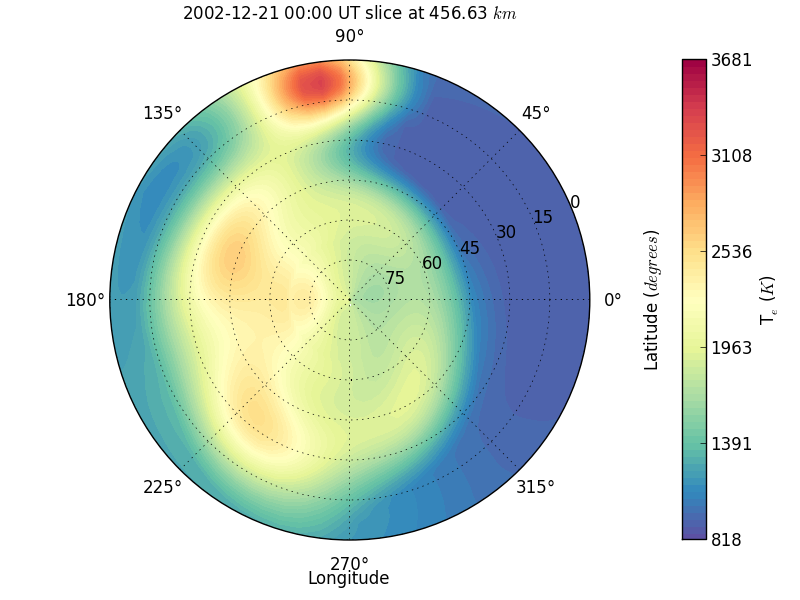
\includegraphics[width=.45 \textwidth]{Figures/plot_single_3D_image_polar.png}
}
\subfigure[]{
\noindent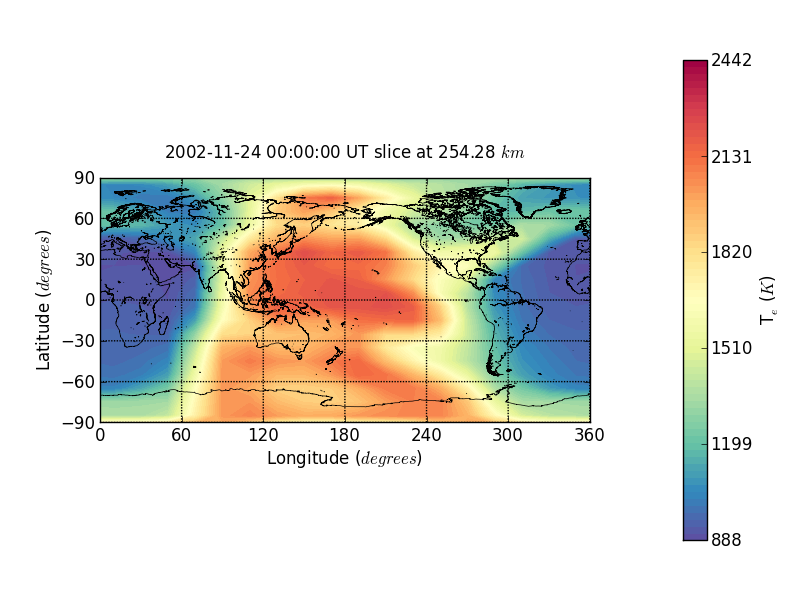
\includegraphics[width=.45 \textwidth]{Figures/plot_single_3D_image_rect.png}
}
\subfigure[]{
\noindent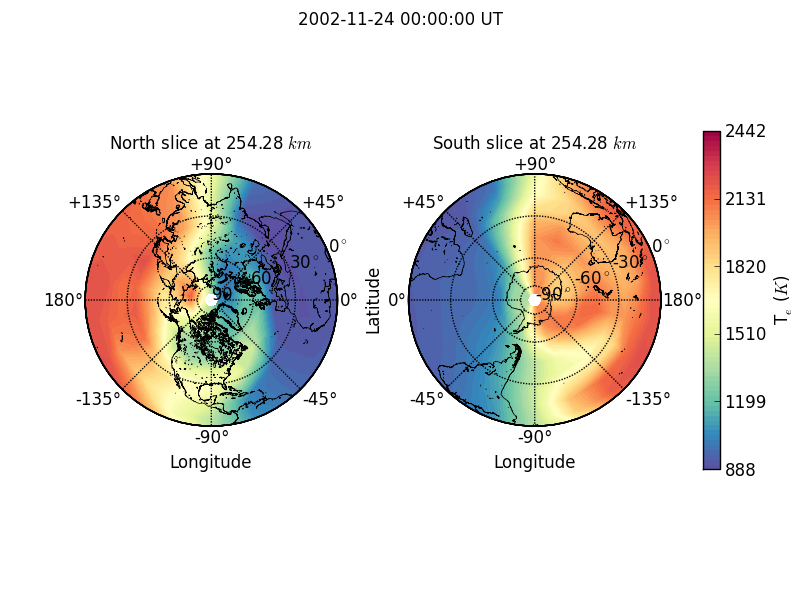
\includegraphics[width=.45 \textwidth]{Figures/plot_single_nsglobal_3D_image.png}
}
\subfigure[]{
\noindent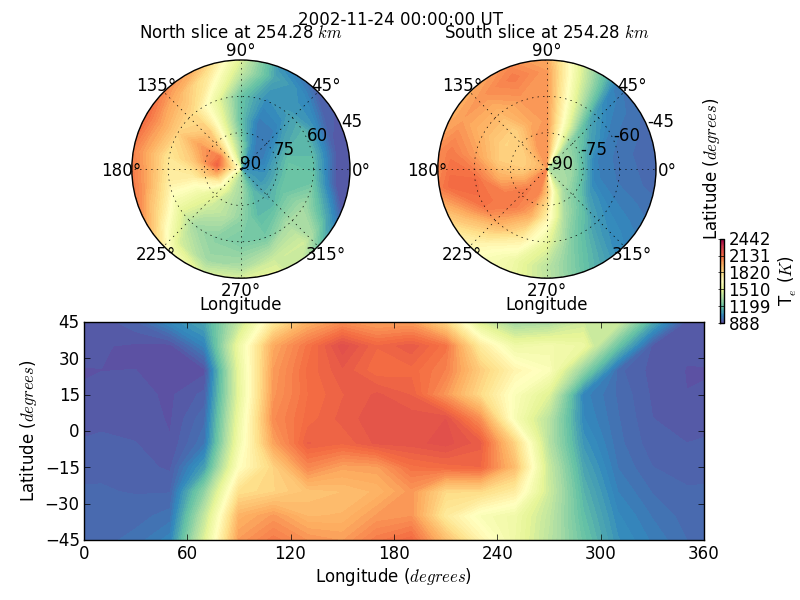
\includegraphics[width=.45 \textwidth]{Figures/plot_global_3D_snapshot.png}
}
\caption{GITM electron temperature at 456.63 $km$ altitude for: (a) northern latitudes, (b) over the entire globe, (c) over the entire globe, as viewed from the poles, and (d) as a global snapshot.}
\label{gitm_3D_global_plots.fig}
\end{center}
\end{figure}

\begin{figure}
\begin{center}
\subfigure[]{
\noindent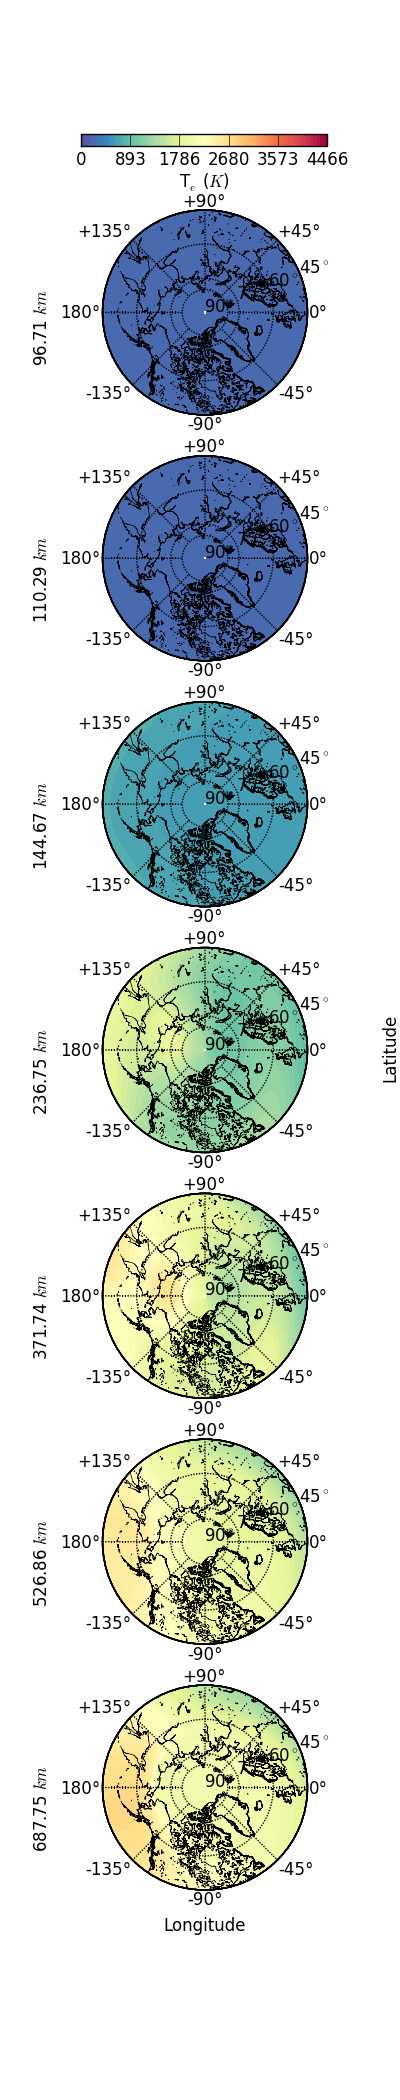
\includegraphics[height=.9 \textheight]{Figures/plot_mult_3D_slices_polar.png}
}
\subfigure[]{
\noindent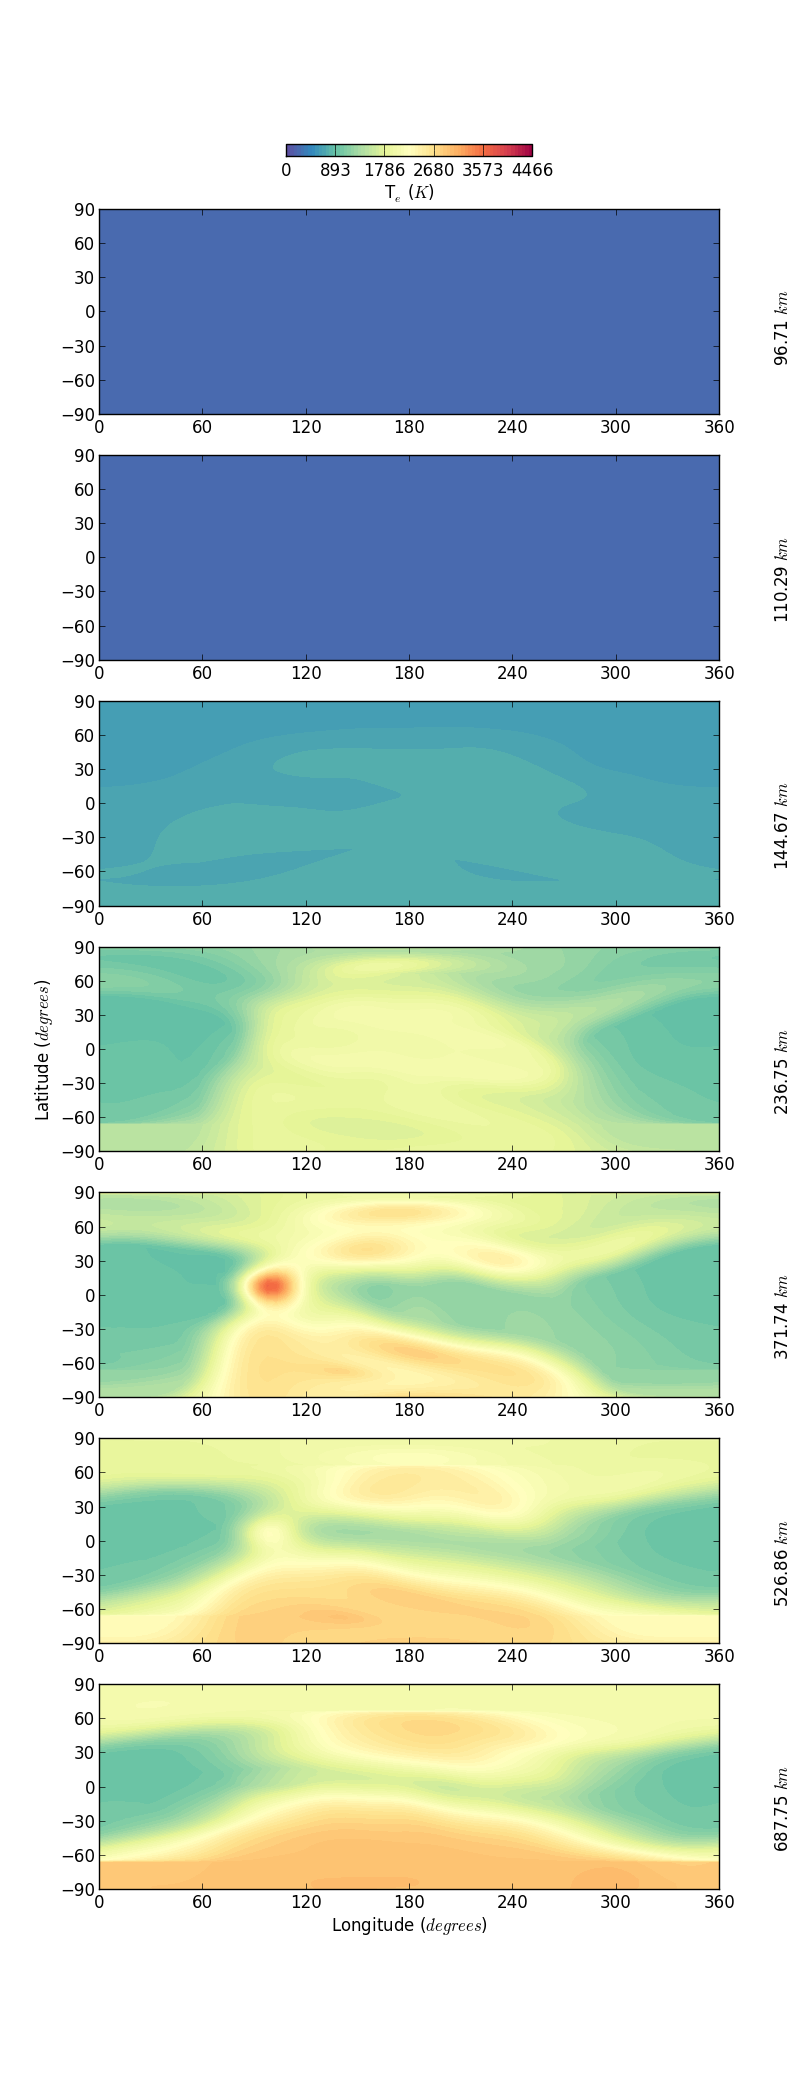
\includegraphics[height=.9 \textheight]{Figures/plot_mult_3D_slices_rect.png}
}
\caption{GITM electron temperature at seven altitude slices for (a) northern latitudes and (b) the entire globe.}
\label{gitm_3D_mult_plots.fig}
\end{center}
\end{figure}

This example shows how to reproduce Figure~\ref{gitm_3D_global_plots.fig}~(a).

\begin{verbatim}
In [1]: import spacepy
In [2]: import gitm
In [3]: import gitm_3D_global_plots as g3d
In [4]: import matplotlib.pyplot as plt
In [5]: plt.ion() # This makes the plotting happen interactively
In [6]: gdata = gitm.GitmBin(`3DALL_t021124_000000.bin')
In [7]: title = "%s UT" % (gdata[`time'])
In [8]: f = g3d.plot_single_3D_image("polar", "eTemperature", gdata, title, 
                                     "example_polar_plot.png", True, 27, 90, 0)
\end{verbatim}

\subsubsection{gitm\_alt\_plots.py}

Routines to build and output GITM output variable linear and contour plots over an altitude range.  Several different standard plot formats are available, and routines useful for creating custom figures are also included.

\begin{itemize}
\item[]{{\bf plot\_single\_alt\_image:}  Creates a single linear or contour altitude plot.}
\item[]{{\bf plot\_mult\_alt\_image:}  Creates a figure with multiple linear or contour altitude plots.}
\item[]{{\bf plot\_alt\_slices:}  Creates a figure with a contour plot showing the altitude dependence of a quantity as a function of latitude or longitude with several linear altitude slices at specified locations.  An example is shown in figure~\ref{gitm_alt_slices.fig}}
\item[]{{\bf plot\_linear\_alt:}  Plots the the linear altitude dependence of a quantity, with altitude on the y-axis.}
\item[]{{\bf plot\_3D\_alt:}  Plots the altitude dependence of a quantity as the function of another spatiotemporal coordinate with the spatiotemporal coordinate on the x-axis, altitude on the y-axis, and the desired quantity as a color contour.}
\end{itemize}

\begin{figure}
\begin{center}
\noindent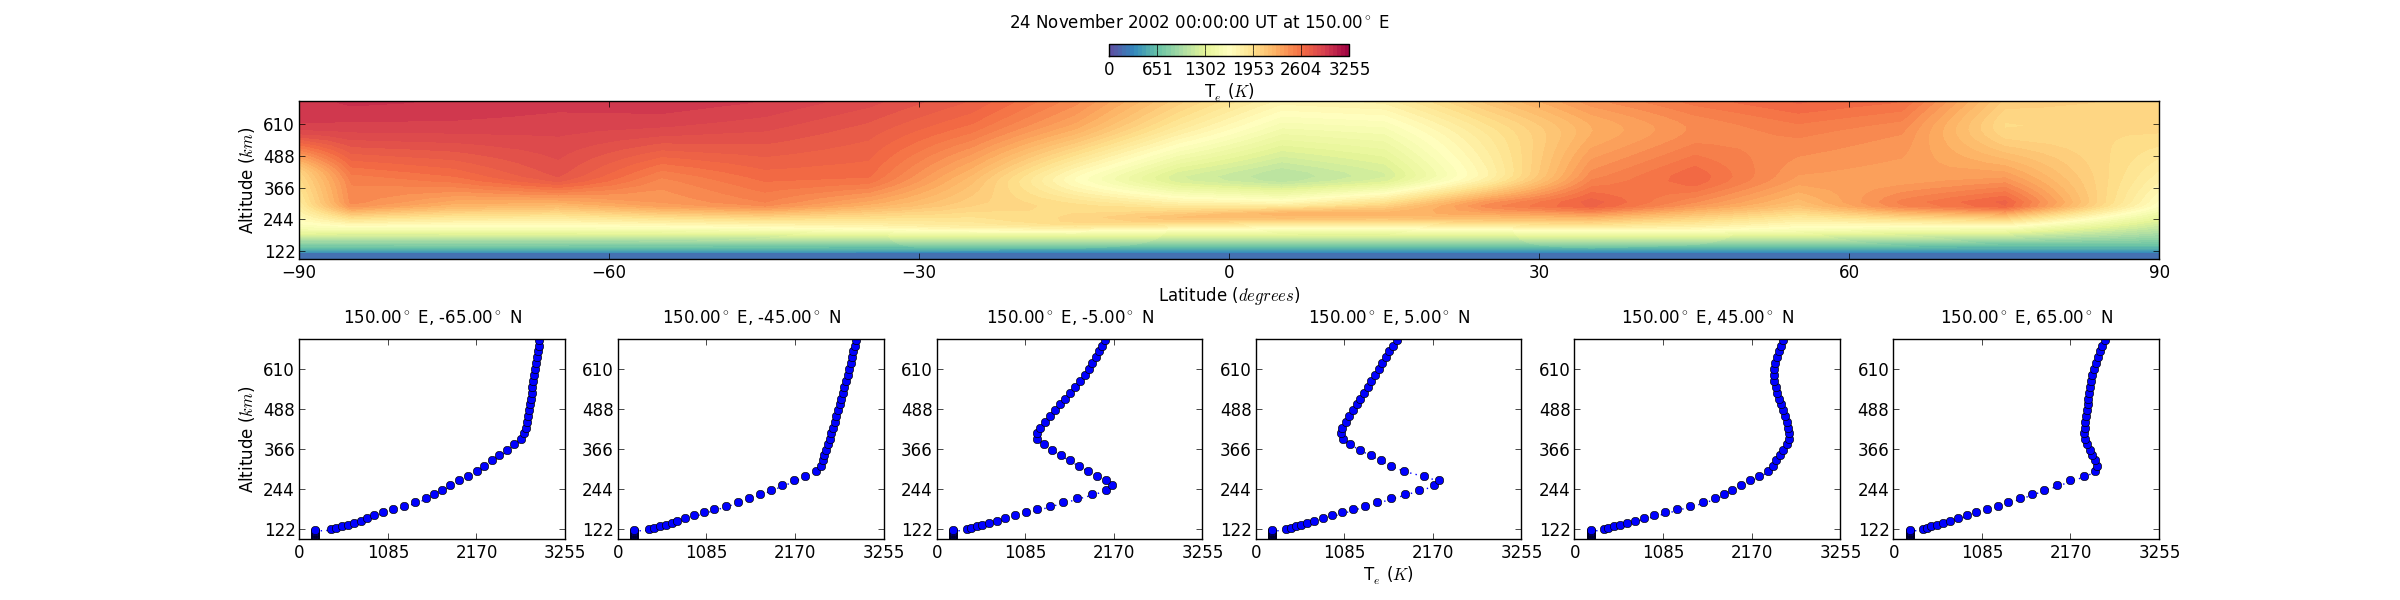
\includegraphics[width=\textwidth]{Figures/gitm_alt_slice_test_Te.png}
\caption{GITM electron temperature at a constant longitude with six latitude slices.}
\label{gitm_alt_slices.fig}
\end{center}
\end{figure}

This example shows how to reproduce Figure~\ref{gitm_alt_slices.fig}.

\begin{verbatim}
In [1]: import spacepy
In [2]: import gitm
In [3]: import gitm_alt_plots as gap
In [4]: import gitm_plot_rout as gpr
In [5]: import matplotlib.pyplot as plt
In [6]: plt.ion() # This makes the plotting happen interactively
In [7]: gdata = gitm.GitmBin(`3DALL_t021124_000000.bin')
In [8]: title = "%s UT" % (gdata[`time'])
In [9]: lat_index = list()
In [10]: lon_index = list()
In [11]: (ilon, ilat) = gpr.find_lon_lat_index(gdata, 150.0, -65.0, "degrees")
In [12]: lon_index.append(ilon)
In [13]: lat_index.append(ilat)
In [14]: (ilon, ilat) = gpr.find_lon_lat_index(gdata, 150.0, -45.0, "degrees")
In [15]: lat_index.append(ilat)
In [16]: (ilon, ilat) = gpr.find_lon_lat_index(gdata, 150.0, -5.0, "degrees")
In [17]: lat_index.append(ilat)
In [18]: (ilon, ilat) = gpr.find_lon_lat_index(gdata, 150.0, 5.0, "degrees")
In [19]: lat_index.append(ilat)
In [20]: (ilon, ilat) = gpr.find_lon_lat_index(gdata, 150.0, 45.0, "degrees")
In [21]: lat_index.append(ilat)
In [22]: (ilon, ilat) = gpr.find_lon_lat_index(gdata, 150.0, 65.0, "degrees")
In [23]: lat_index.append(ilat)
In [24]: f = gap.plot_alt_slices("eTemperature", gdata, lat_index, lon_index, 
                                 title, "example_alt_plot.png")
\end{verbatim}

\subsubsection{gitm\_movie\_script.py}

This is a python script that can be run either from ipython using the command {\tt run gitm\_movie\_script.py} or the command line using the command {\tt python gitm\_movie\_script.py}.  Input to this program is prompted interactively, and includes:

\begin{itemize}
\item{{\tt Ordered list of GITM binary files:}  A list of GITM binary files in chronological order (or whatever other order the movie should be played in).}
\item{{\tt GITM plot type (rectangular, polar, nspolar, snapshot):}  The keyword for the desired plot type.  These are the plot types shown in figure~\ref{gitm_3D_global_plots.fig}, where polar corresponds to panel (a), rectangular to panel (b), nspolar to panel (c), and snapshot to panel (d).}
\item{At this point, the routine enters a while-loop to allow multiple movies to be made for the same list of GITM binary files}
	\begin{itemize}
	\item{{\tt GITM key to plot on z axis (eg Temperature):} The data key corresponding to the data type to plot on the z axis.  A list of data keys can be found by typing `{\tt gdata.keys()}' into ipython after loading one of the listed GITM binaries.}
	\item{{\tt Altitude to plot z value at (eg 250):} Altitude to plot, may be specified in km or m.  For 2D parameters, a value must be entered, but doesn't matter.}
	\item{{\tt Units of altitude (km or m):} Units of altitude entered above.}
	\item{{\tt Use map of Earth? (empty for False):} Enter any value to include a Basemap plot of the earth, enter a carriage return to exclude the map.}
	\item{The latitude limits needed depend on the plot type}
		\begin{itemize}
		\item{{\bf nspolar}  {\tt Polar latitude limit (degrees):} Specify the polar latitude limit (positive, same for both hemispheres).}
		\item{{\bf nspolar} {\tt Equatorial latitude limit (degrees):} Specify the equatorial latitude limit (positive, same for both hemispheres).}
		\item{{\bf snapshot} {\tt Polar latitude limit (degrees):} Specify the polar latitude limit (positive, same for both hemispheres).}
		\item{{\bf polar/rectangular} {\tt Northern latitude limit (degrees):} Specify the northernmost latitude (may be negative).}
     	   	\item{{\bf polar/rectangular} {\tt Southern latitude limit (degrees):} Specify the southernmost latitude (must be smaller/more negative than the northernmost limit)}
		\end{itemize}
		
    \item{{\tt Load another z axis key? (empty for False):} Enter any value to include another movie or, enter a carriage return finish.}
    \end{itemize}
\end{itemize}

With this information, movies with appropriate z-variable ranges will be plot as .png files and combined into a movie using FFmpeg.  The image and movie files will be named using the plot type, z parameter, and altitude to distinguish them.









%Bibliography
\clearpage
\addcontentsline{toc}{chapter}{Bibliography}
\bibliographystyle{chicagoa}
\bibliography{gitm}

\end{document}
